% UG4 Dissertation: Efficient Scheduling for Batched AI Jobs
% Author: Jingsheng
% University of Edinburgh, School of Informatics
% March 2026

\documentclass[logo,bsc,singlespacing,parskip,online]{infthesis}
\usepackage{ugcheck}

% Packages
\usepackage{microtype}
\usepackage[round]{natbib}
\usepackage{graphicx}
\usepackage{amsmath}
\usepackage{amssymb}
\usepackage{algorithm}
\usepackage{algorithmic}
\usepackage{listings}
\usepackage{xcolor}
\usepackage{booktabs}
\usepackage{hyperref}
\usepackage{tikz}
\usepackage{pgfplots}
\pgfplotsset{compat=1.18}
\usetikzlibrary{arrows.meta,positioning,shapes.geometric,fit,backgrounds,calc,patterns,decorations.pathreplacing}

% ── Consistent academic colour palette (soft, muted) ──────────────
\definecolor{cblue}{HTML}{6BA3D6}       % soft blue  – compute / GPU
\definecolor{cbluelight}{HTML}{D6E8F7}  % very light blue – head-node bg
\definecolor{corange}{HTML}{E8915A}     % soft coral  – I/O / loading
\definecolor{corangelight}{HTML}{FDE9D9}% very light orange – worker bg
\definecolor{cgreen}{HTML}{6BAF6B}      % soft green  – storage / cache hit
\definecolor{cgreenlight}{HTML}{E2F0E2} % very light green – storage bg
\definecolor{cpurple}{HTML}{9B72AA}     % soft purple – memory / LoRA
\definecolor{cpurplelight}{HTML}{EDE4F0}% very light purple
\definecolor{camber}{HTML}{E8B84B}      % soft amber  – prefetch overlap
\definecolor{cgray}{HTML}{A6A6A6}       % medium gray – neutral / idle
\definecolor{cgraylight}{HTML}{F2F2F2}  % very light gray – input bg
\definecolor{cred}{HTML}{D96459}        % soft red    – load bars / alerts

% Code listing style
\lstset{
    basicstyle=\ttfamily\small,
    breaklines=true,
    frame=single,
    numbers=left,
    numberstyle=\tiny,
    keywordstyle=\color{blue},
    commentstyle=\color{gray},
    stringstyle=\color{red}
}

\begin{document}
\begin{preliminary}

\title{Efficient Scheduling for Batched AI Jobs: Minimising Makespan through Model Grouping, Johnson's Rule, and Checkpoint Prefetching}

\author{Jingsheng}

\course{Computer Science}

\project{4th Year Project Report}

\date{March 2026}

\abstract{
Large Language Model (LLM) batch workloads---model benchmarking, dataset labelling, and synthetic data generation---submit hundreds of tasks that share common model weights. Existing serverless LLM schedulers treat tasks as independent, causing excessive model switching that dominates total execution time.

This dissertation formalises the batch scheduling problem as a two-machine flow-shop (I/O and GPU computation) and introduces three composable optimisations: (1)~\textbf{model grouping} reduces model switches from $O(n)$ to $O(k)$; (2)~\textbf{Johnson's Rule ordering} sequences model groups to maximise I/O-computation overlap; and (3)~\textbf{checkpoint prefetching} preloads the weights of the next model into CPU pinned memory while the current group executes.

Evaluation on NVIDIA RTX A5000 GPUs shows that model grouping reduces makespan by over 99\% versus FIFO (analytical baseline 42,001s; measured 228.5s for a 501-task batch with three models, 0.6B--32B). Checkpoint prefetching hides the SSD I/O portion of model transitions, reducing per-transition time by $\sim$18s (9.5\% makespan improvement). Johnson's Rule ordering adds a further 20\% by placing model groups optimally for prefetch overlap, yielding a combined 255$\times$ speedup. The shared-aware strategy outperforms FIFO by 60--255$\times$ across measured batch sizes of 99--501 tasks and model sizes of 0.6B--32B, with speedup growing as batch size increases. Prefetching remains effective across storage tiers including 10\,GbE network storage (78.9\% of I/O read latency analytically estimated as hidden), demonstrating the viability of remote storage in production deployments.
}

\maketitle

\newenvironment{ethics}
   {\begin{frontenv}{Research Ethics Approval}{\LARGE}}
   {\end{frontenv}\newpage}

\begin{ethics}
This project was planned in accordance with the Informatics Research
Ethics policy. It did not involve any aspects that required approval
from the Informatics Research Ethics committee.
\end{ethics}

\standarddeclaration

\begin{acknowledgements}
I would like to thank my supervisor for their guidance and feedback throughout this project. I am grateful to the ServerlessLLM team for providing the open-source framework that made this work possible, and to the School of Informatics for providing access to the GPU cluster used for experimental evaluation.
\end{acknowledgements}

\tableofcontents

\end{preliminary}

% ============================================================================
% CHAPTER 1: INTRODUCTION
% ============================================================================

\chapter{Introduction}

Large Language Model (LLM) batch workloads, including model benchmarking, dataset processing, and synthetic data generation, submit thousands of tasks together for offline processing. Unlike online serving, batch tasks are not independent: they share substantial computational structure, including identical model weights and common prompt prefixes, that can be exploited to reduce total execution time.

\section{Motivation}

Consider a model benchmarking scenario: evaluating two LLMs on 10 questions each, totalling 20 tasks. A naive scheduler executes tasks in submission order (ABABAB\ldots), repeatedly loading and evicting model weights. Each model switch takes roughly 100 seconds while each inference requires under a second, so the system spends over 96\% of its time on I/O. Grouping tasks by model (AAAA\ldots BBBB) reduces switches from 10 to~1, cutting execution time by 87\% (Figure~\ref{fig:fifo_vs_grouped}).

Reducing model switches from $O(n)$ to $O(k)$ through grouping provides an order-of-magnitude improvement, but does not eliminate the remaining $O(k)$ model transitions. Checkpoint prefetching hides this residual latency by loading the next model's weights into CPU pinned memory while the current group executes on GPU, exploiting the independence of I/O and GPU computation.

Prefetching effectiveness depends on the \textit{order} in which groups execute: a compute-heavy group provides a large overlap window, while a short group provides little. This structure, where each model group passes through two sequential stages (I/O loading then GPU computation) with the objective of minimising total completion time, is precisely the classical \textit{two-machine flow-shop} problem~\cite{johnson1954optimal}. Johnson's Rule provides the provably optimal group ordering by placing compute-heavy groups first, maximising the overlap window for prefetching.

The three components compose into a complete pipeline: grouping reduces switches from $O(n)$ to $O(k)$, prefetching hides I/O behind computation, and Johnson's Rule maximises overlap. Existing serverless LLM schedulers treat batch tasks as independent, causing excessive model switching and no I/O-computation overlap.

\begin{figure}[htbp]
\centering
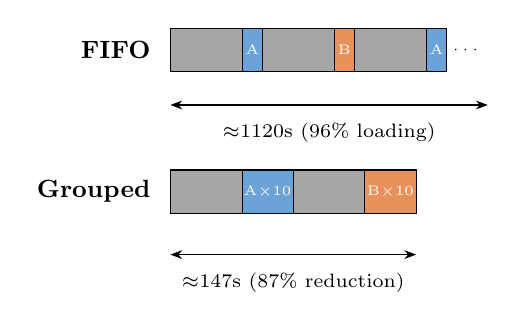
\begin{tikzpicture}[
    xscale=0.065,
    bar/.style={minimum height=0.55cm, anchor=west, font=\tiny, text=white},
    modela/.style={bar, fill=cblue}, modelb/.style={bar, fill=corange},
    loadbar/.style={bar, fill=cgray, text=black},
    label/.style={font=\small, anchor=east},
]
% FIFO  (bars drawn as rectangles to avoid coordinate/minimum-width gap)
\node[label] at (-2, 1.5) {\textbf{FIFO}};
\draw[fill=cgray]   (0,  1.225) rectangle (14, 1.775);
\draw[fill=cblue]   (14, 1.225) rectangle (18, 1.775);
\node[font=\tiny, text=white] at (16, 1.5) {A};
\draw[fill=cgray]   (18, 1.225) rectangle (32, 1.775);
\draw[fill=corange] (32, 1.225) rectangle (36, 1.775);
\node[font=\tiny, text=white] at (34, 1.5) {B};
\draw[fill=cgray]   (36, 1.225) rectangle (50, 1.775);
\draw[fill=cblue]   (50, 1.225) rectangle (54, 1.775);
\node[font=\tiny, text=white] at (52, 1.5) {A};
\node[font=\tiny] at (58, 1.5) {$\cdots$};
\draw[{Stealth[length=1.5mm]}-{Stealth[length=1.5mm]}] (0, 0.8) -- (62, 0.8);
\node[font=\scriptsize] at (31, 0.45) {$\approx$1120s (96\% loading)};
% Grouped
\node[label] at (-2, -0.3) {\textbf{Grouped}};
\draw[fill=cgray]   (0,  -0.575) rectangle (14, -0.025);
\draw[fill=cblue]   (14, -0.575) rectangle (24, -0.025);
\node[font=\tiny, text=white] at (19, -0.3) {A$\times$10};
\draw[fill=cgray]   (24, -0.575) rectangle (38, -0.025);
\draw[fill=corange] (38, -0.575) rectangle (48, -0.025);
\node[font=\tiny, text=white] at (43, -0.3) {B$\times$10};
\draw[{Stealth[length=1.5mm]}-{Stealth[length=1.5mm]}] (0, -1.1) -- (48, -1.1);
\node[font=\scriptsize] at (24, -1.45) {$\approx$147s (87\% reduction)};
\end{tikzpicture}
\caption{FIFO vs Model-Grouped scheduling for 20 tasks with 2 models. FIFO incurs 10 switches (each $\sim$108s); grouping requires only 1 switch.}
\label{fig:fifo_vs_grouped}
\end{figure}

\section{Problem Definition}

A batch is submitted as a JSONL file where each line specifies one task: the target model, the prompt, and generation parameters. The example below shows a small multi-model batch typical of model benchmarking.

\begin{lstlisting}[language={},basicstyle=\ttfamily\small,frame=single,numbers=none]
{"custom_id":"t1","method":"POST","url":"/v1/chat/completions",
 "body":{"model":"Qwen/Qwen3-0.6B",
         "messages":[{"role":"user","content":"Summarise the paper."}],
         "max_tokens":256}}
{"custom_id":"t2","method":"POST","url":"/v1/chat/completions",
 "body":{"model":"Qwen/Qwen3-8B",
         "messages":[{"role":"user","content":"Summarise the paper."}],
         "max_tokens":256}}
{"custom_id":"t3","method":"POST","url":"/v1/chat/completions",
 "body":{"model":"Qwen/Qwen3-0.6B",
         "messages":[{"role":"user","content":"Translate to French."}],
         "max_tokens":128}}
\end{lstlisting}

Tasks \texttt{t1} and \texttt{t3} share the same model and can execute consecutively without reloading; \texttt{t2} requires a model switch. The API follows the OpenAI Batch API specification \citep{openai_batch_api}: clients submit a file via \texttt{POST /v1/files}, create a batch via \texttt{POST /v1/batches}, and poll via \texttt{GET /v1/batches/\{id\}}. Results are written to an output JSONL file keyed by \texttt{custom\_id}.

\textbf{Input:}
\begin{itemize}
\item A batch of $n$ tasks $B = \{t_1, t_2, \ldots, t_n\}$
\item Each task $t_i = (m_i, p_i, \theta_i)$ where $m_i$ is the model, $p_i$ is the prompt, and $\theta_i$ are generation parameters
\item A cluster of $k$ GPU workers $W = \{w_1, w_2, \ldots, w_k\}$
\item Each worker can load at most one model at a time, with loading latency $L_{load}(m)$
\item Task inference latency is $L_{infer}(t_i)$
\end{itemize}

\textbf{Sharing Relationships:}
\begin{itemize}
\item \textbf{Model Sharing}: If $m_i = m_j$, tasks $t_i$ and $t_j$ can share loaded model weights, avoiding redundant loading. This is the primary sharing relationship exploited in this work.
\item \textbf{Prefix Sharing}: If $\text{prefix}(p_i) = \text{prefix}(p_j)$, tasks can benefit from inference engine cache reuse. This is a secondary sharing relationship identified but not exploited in this work (see Chapter~\ref{ch:future}).
\end{itemize}

\textbf{Optimisation Objective:}
$$\text{Minimise } C_{max} = \max_{i \in \{1,...,n\}} \text{completion\_time}(t_i)$$

That is, minimise the makespan: the time at which the last task completes.

\textbf{Constraints:}
\begin{itemize}
\item Each worker loads at most one model at a time (single-model constraint)
\item Model switching incurs $L_{load}$ overhead (cold start penalty)
\item Worker count $k$ can be adjusted via auto-scaling
\end{itemize}

\section{Research Questions}

Three research questions are addressed:

\begin{description}
\item[RQ1:] How can shared structure (shared models) in a batch be discovered and exploited to reduce makespan? Specifically, how does model grouping compare to naive FIFO scheduling?

\item[RQ2:] Can the batch scheduling problem be modelled as a two-machine flow-shop (I/O and compute), and does Johnson's Rule provide an effective ordering of model groups to maximise I/O-computation overlap via checkpoint prefetching?

\item[RQ3:] How do different scheduling strategies (FIFO, Model Grouping, Shared-Aware with prefetching) compare across varying batch sizes, model sizes, and storage tiers (local SSD, RAID, network storage)?
\end{description}

\section{Contributions}

Five contributions are made:

\begin{enumerate}
\item \textbf{Two-Machine Flow-Shop Formulation}: The batch scheduling problem is modelled as a classical two-machine flow-shop where Machine~A is I/O (loading model weights) and Machine~B is GPU computation, enabling Johnson's Rule for provably optimal model group ordering.

\item \textbf{Shared-Aware Scheduling Algorithm}: An algorithm that discovers model sharing relationships within a batch, groups tasks by model to reduce switches from $O(n)$ to $O(k)$, and applies Johnson's Rule to order groups for maximal I/O-computation overlap.

\item \textbf{Checkpoint Prefetching Mechanism}: A prefetching policy using the pinned memory pool of ServerlessLLM to preload the next model's weights while the current group executes, hiding I/O latency through pipelining.

\item \textbf{Network-Aware Prefetching Extension}: Analysis and evaluation of prefetching across storage tiers including RAID-0, 10\,GbE NFS, and 100\,GbE NFS, demonstrating that the prefetch architecture generalises to network-attached storage.

\item \textbf{OpenAI-Compatible Batch API}: An OpenAI-compatible batch REST API extended for multi-model batches, enabling clients to submit heterogeneous task lists with a single request and receive results asynchronously.
\end{enumerate}

The project contributed approximately 3,500 lines of new Python code to the existing ServerlessLLM framework ($\sim$15K LoC).

\section{Scope and Boundaries}

This work focuses strictly on cluster-level scheduling. The inference engine is neither modified nor optimised; KV cache management, prefill-decode separation, continuous batching internals, and GPU kernel optimisations are out of scope. The scheduler decides which tasks to execute, in what order, and on which workers; vLLM handles the computation. Scheduler-level optimisations are complementary to engine-level optimisations and require no engine modification.


% ============================================================================
% CHAPTER 2: BACKGROUND
% ============================================================================

\chapter{Background}


\section{Transformer-Based LLM Inference}

LLMs are built on the transformer architecture \citep{vaswani2017attention}, generating tokens autoregressively via a compute-bound prefill phase ($O(L^2)$ attention) followed by a memory-bandwidth-bound decode phase (one token per step). Modern LLMs range from 0.5B to 405B parameters \citep{brown2020language, touvron2023llama}; an 8B model requires $\sim$15\,GB in FP16 and a 70B model $\sim$140\,GB. Loading weights from storage takes 80--120 seconds for an 8B model from SSD.

vLLM \citep{kwon2023efficient} introduced continuous batching (iteration-level scheduling), inserting new requests at every decode step to maintain near-full GPU utilisation within a single loaded model. It does not address switching between models. Tensor parallelism \citep{shoeybi2019megatron} shards weight matrices across multiple GPUs for models exceeding a single GPU's VRAM; this work assumes each model fits within one GPU, and tensor parallelism can be combined with the proposed scheduler when needed.

\section{KV Cache and Prefix Caching}
\label{sec:bg_kv_cache}

Inference engines cache key-value tensors to avoid redundant computation. vLLM manages the KV cache in fixed-size blocks via PagedAttention \citep{kwon2023efficient}, eliminating fragmentation. When requests share a prompt prefix, KV blocks can be computed once and reused \citep{zheng2024sglang}, though interleaving different prefixes causes eviction. This prefix-level optimisation is complementary to model grouping but is not exploited here (see Chapter~\ref{ch:future}).

\section{GPU Memory Hierarchy and Pinned Memory}
\label{sec:bg_pinned_memory}

Loading model weights proceeds in two stages: SSD to CPU RAM via filesystem I/O (2--5\,GB/s on NVMe), then CPU RAM to GPU VRAM via PCIe DMA (16--32\,GB/s on PCIe Gen4 x16). The CPU-to-GPU step is faster with pinned (page-locked) memory, allocated via \texttt{cudaHostAlloc} or \texttt{cudaHostRegister} \citep{cuda_guide2024}, which enables direct DMA without intermediate copies. The sllm-store component of ServerlessLLM \citep{fu2024serverlessllm} pre-allocates a pinned memory pool at startup; weights are loaded into this pool via multi-threaded I/O and transferred to the GPU via DMA, achieving near-peak PCIe bandwidth.

\section{Serverless Computing and Cold Starts}

Serverless functions suffer from cold starts: the latency of initialising a new instance \citep{shahrad2020serverless}. For LLM inference these are severe; loading an 8B model takes 80--120\,s, some 100--200$\times$ the per-request inference latency. ServerlessLLM \citep{fu2024serverlessllm} mitigates this through locality-enhanced scheduling that routes inference to nodes with locally cached checkpoints.

\section{ServerlessLLM Architecture}
\label{sec:bg_serverlessllm}

ServerlessLLM \citep{fu2024serverlessllm} is an open-source serverless LLM inference framework designed for low-latency model loading. Its four components are: a \textbf{Head Node}, which receives requests via an API gateway, maintains deployment state in SQLite, and dispatches tasks via a Router; \textbf{Workers (Pylets)}, GPU nodes each running vLLM for inference with Pylet managing instance lifecycle; \textbf{sllm-store}, a C++ storage daemon per worker managing a pinned memory pool and providing gRPC endpoints for model loading (\texttt{LoadModelAsync}, \texttt{RegisterModel}) with multi-threaded I/O to saturate SSD bandwidth \citep{grpc2024}; and an \textbf{AutoScaler}, which reactively adjusts vLLM instance count based on queue depth.

The existing scheduler targets online serving via round-robin assignment, with two limitations for batch workloads: tasks are assigned without considering shared models, causing excessive switching, and scaling is reactive rather than proactive, causing cold starts at batch start.

\section{Storage Hierarchy and Network-Attached Model Repositories}
\label{sec:bg_storage_hierarchy}

The storage tier determines I/O time $a_i$ in the two-machine flow-shop formulation, directly affecting prefetching effectiveness. Local NVMe SSDs provide 2--5\,GB/s; RAID-0 (4$\times$) aggregates to 8--12\,GB/s. Remote storage (S3, GCS, NFS, Lustre) provides unlimited capacity and replication at 1.2--12\,GB/s. Production systems use local SSD as a cache and remote storage as the source of truth. Scheduling implications are analysed in Section~\ref{sec:prefetch_storage_tiers}.

\section{Makespan Minimisation}
\label{sec:bg_makespan}

Makespan minimisation assigns $n$ jobs to $m$ machines to minimise $C_{\max}$ \citep{pinedo2016scheduling}. The Longest Processing Time (LPT) rule \citep{graham1966bounds} gives a $(4/3 - 1/(3m))$-approximation for identical machines. LLM batch scheduling has sequence-dependent setup times (model loading: $\sim$100\,s per switch, zero for same-model jobs), making the general problem NP-hard \citep{pinedo2016scheduling}.

\subsection{Johnson's Rule for Two-Machine Flow-Shops}
\label{sec:bg_johnsons_rule}

Johnson's Rule \citep{pinedo2016scheduling} solves the two-machine flow-shop optimally: given $n$ jobs processed first on Machine~A then Machine~B, find the permutation minimising makespan. Partition jobs into $S_1 = \{j : a_j \leq b_j\}$ (compute-heavy, sorted by $a_j$ ascending) and $S_2 = \{j : a_j > b_j\}$ (I/O-heavy, sorted by $b_j$ descending); the optimal sequence is $S_1$ followed by $S_2$. Compute-heavy jobs execute first because their prolonged Machine~B execution conceals the loading of the next job on Machine~A; I/O-heavy jobs are placed last since fewer subsequent jobs remain to stall while their loading completes.

Machine~A is the I/O stage (loading weights from SSD to CPU pinned memory), Machine~B is the compute stage (GPU inference for all tasks in a group), and each job is a model group. This mapping is formalised in Chapter~4.


% ============================================================================
% CHAPTER 2B: RELATED WORK
% ============================================================================

\chapter{Related Work}


\section{LLM Batch Workloads}

LLM batch workloads take three common forms: model benchmarking (evaluating candidates on suites such as MMLU \citep{hendrycks2020measuring}, HumanEval \citep{chen2021evaluating}, and MT-Bench \citep{zheng2023judging}, with high prompt overlap but diverse model identities); dataset processing (large-scale labelling, translation, or summarisation with a single model); and synthetic data generation (template-based prompts exhibiting both model and prefix overlap).

The OpenAI Batch API \citep{openai_batch_api} supports up to 50,000 tasks per batch with 50\% cost savings; AWS Bedrock Batch \citep{aws_bedrock_batch} provides similar functionality. Both are closed-source, single-model only, and do not expose scheduling policies.

\section{ML Serving Systems}

Clipper \citep{crankshaw2017clipper} provides adaptive batching for online latency SLOs. INFaaS \citep{romero2021infaas} automates model variant selection, treating switching as a configuration change. Clockwork \citep{gujarati2020serving} achieves predictable DNN serving through profiling, but its deterministic timing assumption does not extend to autoregressive LLMs. AlpaServe \citep{li2023alpaserve} uses statistical multiplexing with model parallelism but does not reorder tasks across models. vLLM \citep{kwon2023efficient} combines PagedAttention, continuous batching, and tensor parallelism for single-model serving; multi-model batches still require sequential loads between groups. Orca \citep{yu2022orca} introduced iteration-level scheduling within a single model. None of these systems address cross-model task reordering for makespan minimisation.

\section{Data-Locality and Model-Aware Scheduling}

MapReduce \citep{dean2008mapreduce} and Spark \citep{zaharia2010spark} schedule tasks on nodes holding the input data; for LLM inference the analogue is routing to nodes holding model weights. Borg \citep{verma2015large} and Kubernetes \citep{kubernetes2024} provide affinity-based cluster scheduling without model-specific optimisations. Database multi-query optimisers identify common subexpressions across queries \citep{sellis1988multiple}, inspiring the present approach of discovering shared structure before optimising execution order. ServerlessLLM \citep{fu2024serverlessllm} provides locality-enhanced scheduling with local SSD caching but does not reorder tasks by model or prefix.

\section{Prefetching and Pipelining}

OS-level prefetching uses sequential access patterns \citep{patterson2013computer}. DeepSpeed-Inference \citep{aminabadi2022deepspeed} prefetches transformer layers during inference, overlapping CPU-to-GPU transfer with computation; FlexGen \citep{sheng2023flexgen} pipelines model offloading across CPU, GPU, and disk for memory-constrained inference; CheckFreq \citep{mohan2021checkfreq} analyses checkpoint I/O costs during training. No existing system performs checkpoint prefetching at the cluster scheduler level. This work introduces task-group-level prefetching, where the scheduler predicts the next model from the execution plan and begins loading it before the current group completes.

\section{Summary and Research Gap}

\begin{table}[htbp]
\centering
\caption{Comparison of scheduling approaches for LLM inference}
\label{tab:related_work_comparison}
\begin{tabular}{lccccc}
\toprule
System & Batch & Model & Prefix & Prefetch & Open \\
       & Support & Grouping & Sorting & & Source \\
\midrule
Orca \citep{yu2022orca} & \texttimes & \texttimes & \texttimes & \texttimes & \texttimes \\
Clipper \citep{crankshaw2017clipper} & \texttimes & \texttimes & \texttimes & \texttimes & \checkmark \\
AlpaServe \citep{li2023alpaserve} & \texttimes & Placement & \texttimes & \texttimes & \checkmark \\
ServerlessLLM \citep{fu2024serverlessllm} & \texttimes & Locality & \texttimes & \texttimes & \checkmark \\
OpenAI Batch \citep{openai_batch_api} & \checkmark & N/A$^*$ & ? & ? & \texttimes \\
\textbf{This work} & \checkmark & \checkmark & \texttimes$^\dagger$ & \checkmark & \checkmark \\
\bottomrule
\multicolumn{6}{l}{\scriptsize $^*$OpenAI Batch API is single-model only, so model grouping is not applicable.} \\
\multicolumn{6}{l}{\scriptsize $^\dagger$Prefix-aware task ordering is identified as future work; only model-level grouping is implemented.}
\end{tabular}
\end{table}

Existing systems either focus on online serving or provide batch APIs without shared-structure-aware scheduling. This work fills that gap with a cluster-level scheduler that discovers model sharing, applies Johnson's Rule for optimal group ordering, and uses checkpoint prefetching to hide loading latency.




% ============================================================================
% CHAPTER 3: DESIGN & IMPLEMENTATION
% ============================================================================

\chapter{Design and Implementation}

The shared-aware scheduling system has four components: shared-structure analysis discovering model sharing; a two-machine flow-shop formulation with Johnson's Rule for optimal group ordering; checkpoint prefetching to hide model loading latency; and multi-GPU load balancing.

\section{System Architecture Overview}

The system extends the ServerlessLLM head node with three new components: the BatchScheduler (model grouping and Johnson's Rule ordering), the StorageManager (checkpoint prefetching into the pinned memory pool), and a batch-aware AutoScaler integration, all operating at cluster scheduler level without inference engine modifications. A SQLite database (\texttt{state.db}) stores batch jobs, task status, and deployment configuration; the Router reads healthy worker endpoints from it. Data flow: (1)~the user submits a batch via the API Gateway; (2)~the BatchScheduler groups tasks, applies Johnson's Rule, persists job state, and feeds ordered tasks to the Router; (3)~the Router dispatches tasks to vLLM workers; (4)~the StorageManager prefetches the next model's weights while the current group executes; (5)~the AutoScaler adjusts instance count.

Figure~\ref{fig:system_arch} illustrates the system architecture.

\begin{figure}[htbp]
\centering
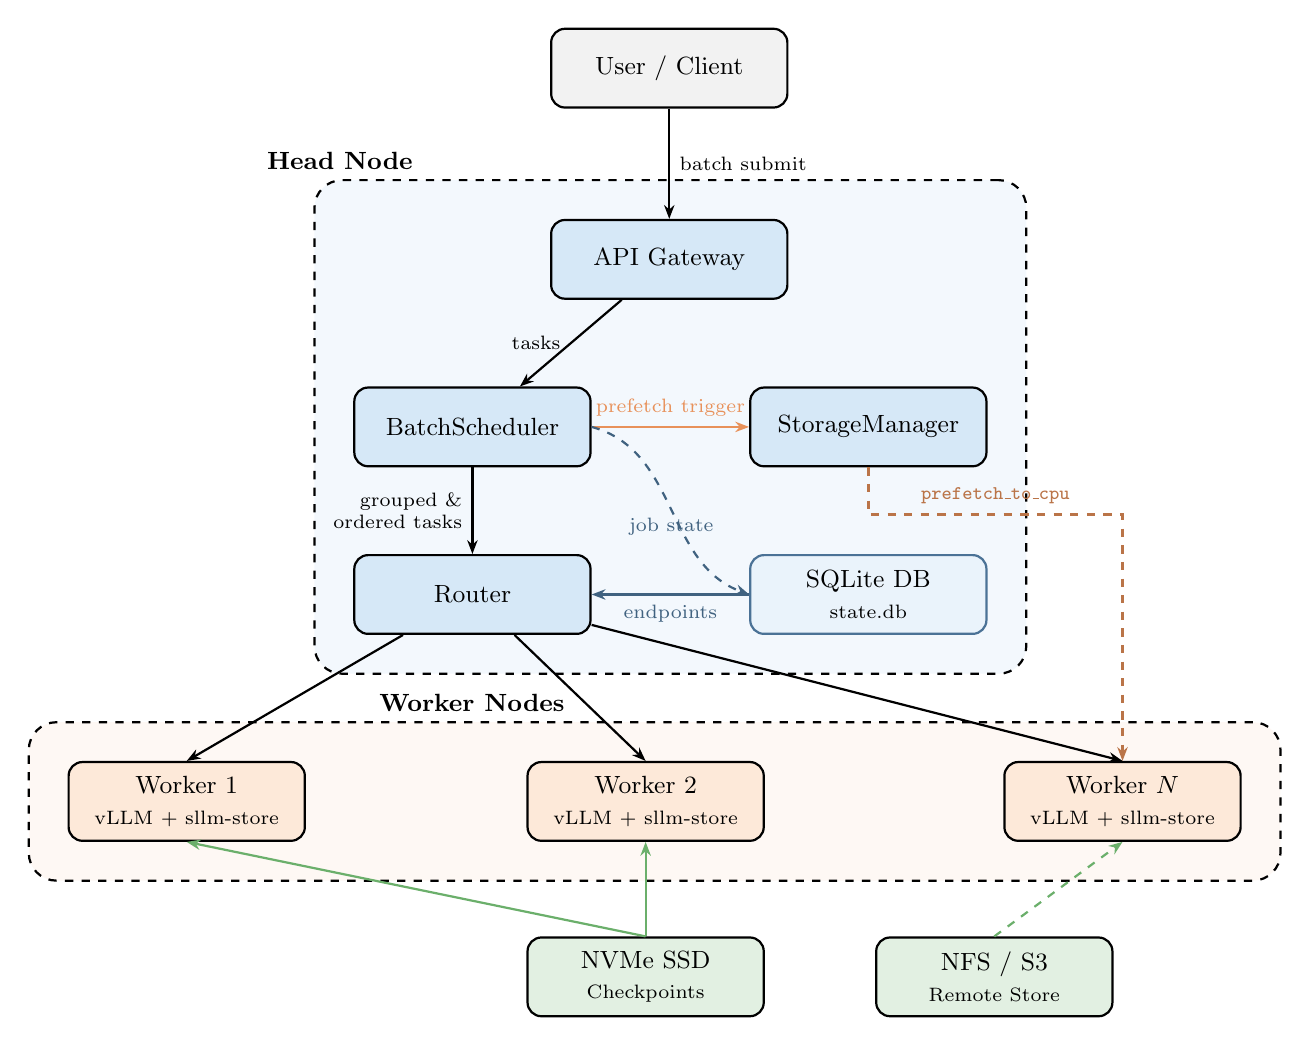
\begin{tikzpicture}[
    box/.style={draw, rounded corners=5pt, minimum width=3.0cm, minimum height=1.0cm,
                font=\small, align=center, thick},
    headbox/.style={box, fill=cbluelight},
    workerbox/.style={box, fill=corangelight},
    storagebox/.style={box, fill=cgreenlight},
    dbbox/.style={box, fill=cbluelight!50, draw=cblue!70!black},
    arr/.style={-{Stealth[length=5pt]}, thick},
    region/.style={draw, dashed, rounded corners=10pt, inner sep=14pt, thick},
]

% User / Client
\node[box, fill=cgraylight] (user) {User / Client};

% Head Node — gateway centred at top; 2×2 grid below
\node[headbox, below=1.4cm of user] (gateway) {API Gateway};

% Row 2: scheduler (left) and storage_mgr (right), symmetric about x=0
\node[headbox, below=1.1cm of gateway, xshift=-2.5cm] (scheduler) {BatchScheduler};
\node[headbox, right=2.0cm of scheduler]              (storage_mgr) {StorageManager};

% Row 3: router under scheduler, db under storage_mgr
\node[headbox, below=1.1cm of scheduler] (router) {Router};
\node[dbbox,   below=1.1cm of storage_mgr] (db) {SQLite DB\\{\scriptsize state.db}};

% Head node background
\begin{scope}[on background layer]
\node[region, fill=cbluelight!30, fit=(gateway)(scheduler)(storage_mgr)(router)(db),
      label={[font=\small\bfseries]above left:Head Node}] (headregion) {};
\end{scope}

% Worker nodes
\node[workerbox, below left=1.6cm and 0.6cm of router] (w1) {Worker 1\\{\scriptsize vLLM + sllm-store}};
\node[workerbox, below=1.6cm of router, xshift=2.2cm]  (w2) {Worker 2\\{\scriptsize vLLM + sllm-store}};
\node[workerbox, below right=1.6cm and 0.2cm of db]    (wn) {Worker $N$\\{\scriptsize vLLM + sllm-store}};

% Worker region background
\begin{scope}[on background layer]
\node[region, fill=corangelight!30, fit=(w1)(w2)(wn),
      label={[font=\small\bfseries]above left:Worker Nodes}] (workerregion) {};
\end{scope}

% Storage
\node[storagebox, below=1.2cm of w2] (ssd) {NVMe SSD\\{\scriptsize Checkpoints}};
\node[storagebox, right=1.4cm of ssd] (nfs) {NFS / S3\\{\scriptsize Remote Store}};

% ── Arrows ──

% Request path
\draw[arr] (user)      -- node[right, font=\scriptsize] {batch submit} (gateway);
\draw[arr] (gateway)   -- node[left,  font=\scriptsize] {tasks} (scheduler);

% Scheduler → StorageManager (prefetch trigger)
\draw[arr, corange] (scheduler) -- node[above, font=\scriptsize] {prefetch trigger} (storage_mgr);

% Scheduler → Router (ordered tasks)
\draw[arr] (scheduler) -- node[left, font=\scriptsize, align=right] {grouped \&\\ordered tasks} (router);

% Scheduler → DB (diagonal through centre of head node — clear of all boxes)
\draw[arr, cblue!60!black, dashed]
    (scheduler.east) to[out=-15, in=160]
    node[midway, below, font=\scriptsize] {job state} (db.west);

% DB → Router (horizontal, same row)
\draw[arr, cblue!60!black]
    (db.west) -- node[below, font=\scriptsize] {endpoints} (router.east);

% StorageManager → Worker N (prefetch_to_cpu): straight down then right
\draw[arr, corange!80!black, dashed, line width=1.2pt]
    (storage_mgr.south) -- ++(0, -0.6)
    -| node[pos=0.25, above, font=\scriptsize] {\texttt{prefetch\_to\_cpu}} (wn.north);

% Router → Workers
\draw[arr] (router) -- (w1.north);
\draw[arr] (router) -- (w2.north);
\draw[arr] (router) -- (wn.north);

% Storage → Workers
\draw[arr, cgreen]        (ssd.north) -- (w1.south);
\draw[arr, cgreen]        (ssd.north) -- (w2.south);
\draw[arr, cgreen, dashed] (nfs.north) -- (wn.south);

\end{tikzpicture}
\caption{System architecture. The BatchScheduler groups tasks by model, applies Johnson's Rule ordering, and persists job state to a SQLite database. The Router queries the same database for healthy worker endpoints. The StorageManager triggers asynchronous checkpoint prefetching (\texttt{prefetch\_to\_cpu}) to worker nodes ahead of execution. Workers run vLLM with sllm-store for pinned-memory checkpoint management.}
\label{fig:system_arch}
\end{figure}

\section{Problem Analysis: Shared Structure in Batches}

\subsection{Model Sharing Analysis}

Batch workloads exhibit substantial model sharing: in benchmarking, multiple tasks use the same model with different prompts; in dataset processing, all tasks share one model. With arbitrary ordering across $k$ distinct models, the system incurs $O(n)$ switches in the worst case, each requiring eviction and reload (80--120 seconds for an 8B model). Grouping reduces switches to $O(k)$; for 20 interleaved tasks across two models, this eliminates $9 \times 108 = 972$ seconds of overhead. Since $L_{load}$ is 100--200$\times$ larger than $L_{infer}$, minimising switches has first-order impact on makespan.

\subsection{Prefix Sharing Analysis}

Batch tasks often share prompt prefixes (RAG contexts, few-shot examples, system prompts). Prefix caching reduces prefill time from $\sim$2\,s to $\sim$0.05\,s, but model switching costs 80--120\,s, making model grouping the first-order optimisation. Prefix-aware ordering within groups is left as future work (Chapter~\ref{ch:future}).

\section{Shared-Aware Scheduling Algorithm}


\subsection{Phase 1: Model Grouping}

Given a batch $B = \{t_1, t_2, \ldots, t_n\}$, tasks are grouped by model to minimise model switches:

\begin{algorithmic}
\STATE $groups \gets \{\}$
\FOR{$t_i \in B$}
  \STATE $m \gets t_i.model$
  \IF{$m \notin groups$}
    \STATE $groups[m] \gets []$
  \ENDIF
  \STATE $groups[m].\text{append}(t_i)$
\ENDFOR
\end{algorithmic}

This produces $k$ model groups $\{G_1, \ldots, G_k\}$ where each $G_i$ contains all tasks for one model, reducing switches from $O(n)$ to $O(k)$.

\subsection{Phase 2: Johnson's Rule Ordering}
\label{sec:johnsons_rule}

Model groups map naturally to a two-machine flow-shop: each group is first loaded from storage (Machine~A: I/O) then executed on GPU (Machine~B: compute). With checkpoint prefetching, loading the next group overlaps with executing the current one. Johnson's Rule determines the group ordering that minimises makespan.

For each model group $G_i$, two times are estimated:
\begin{itemize}
\item $a_i$ (I/O time): the time to load model $m_i$'s checkpoint from SSD to CPU pinned memory, estimated as $a_i = \text{checkpoint\_size}(m_i) / \text{NVMe\_bandwidth}$.
\item $b_i$ (compute time): the time to execute all tasks in $G_i$ on GPU, estimated as $b_i = |G_i| \times \tau_{base} \times (\text{model\_size}(m_i) / \text{base\_model\_size})$, where $\tau_{base}$ is the base per-task inference time.
\end{itemize}

Checkpoint size is determined by scanning the model directory for weight files (\texttt{.safetensors}, \texttt{.bin}, \texttt{.pt}), cached after the initial scan. Figure~\ref{fig:flowshop_mapping} illustrates this mapping.

\begin{figure}[htbp]
\centering
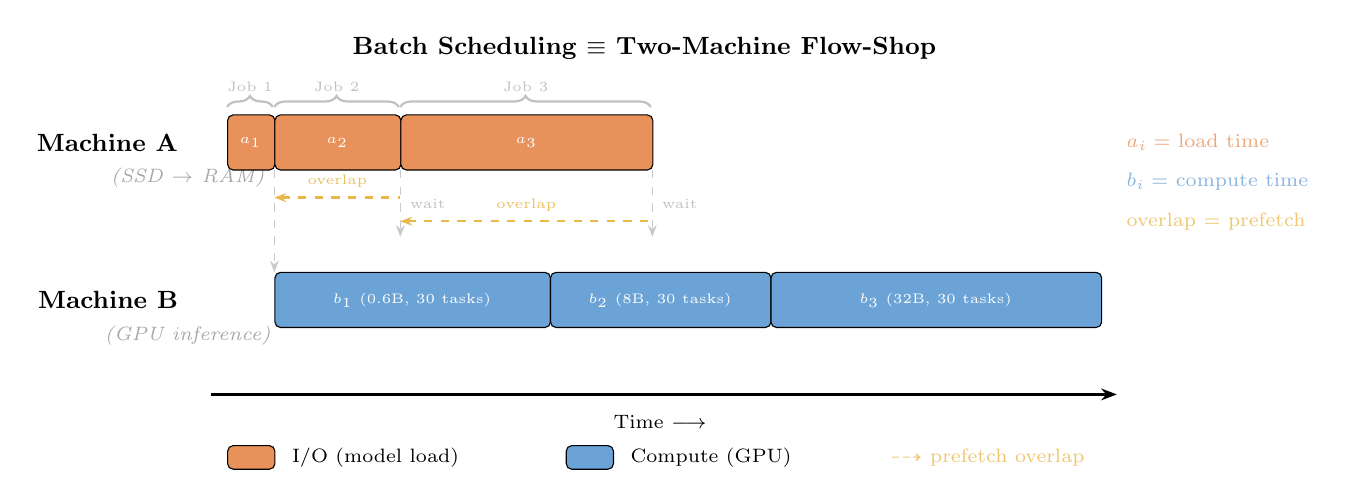
\begin{tikzpicture}[
    node distance=0.4cm,
    mach/.style={draw, rounded corners=2pt, minimum height=0.7cm, anchor=west,
                 font=\scriptsize, text=white, line width=0.4pt},
    io/.style={mach, fill=corange},
    gpu/.style={mach, fill=cblue},
    idle/.style={mach, fill=cgray!20, text=cgray!70, dashed, draw=cgray!50},
    label/.style={font=\small, anchor=east},
    annot/.style={font=\scriptsize\itshape, text=cgray},
    brace/.style={decorate, decoration={brace, amplitude=4pt}},
]

% Title
\node[font=\small\bfseries] at (5.5, 5.0) {Batch Scheduling $\equiv$ Two-Machine Flow-Shop};

% Machine labels
\node[label] at (-0.3, 3.8) {\textbf{Machine A}};
\node[annot] at (-0.3, 3.35) {(SSD $\to$ RAM)};
\node[label] at (-0.3, 1.8) {\textbf{Machine B}};
\node[annot] at (-0.3, 1.35) {(GPU inference)};

% === Machine A: I/O jobs (sequential, no overlap) ===
\node[io, minimum width=0.6cm] (io1) at (0.2, 3.8) {};
\node[font=\tiny, text=white] at (0.5, 3.8) {$a_1$};
\node[io, minimum width=1.6cm] (io2) at (0.8, 3.8) {};
\node[font=\tiny, text=white] at (1.6, 3.8) {$a_2$};
\node[io, minimum width=3.2cm] (io3) at (2.4, 3.8) {};
\node[font=\tiny, text=white] at (4.0, 3.8) {$a_3$};

% === Machine B: GPU compute (each starts after its I/O finishes) ===
% Job 1: starts after io1 finishes (0.8), compute 3.5cm
\node[gpu, minimum width=3.5cm] (gpu1) at (0.8, 1.8) {};
\node[font=\tiny, text=white] at (2.55, 1.8) {$b_1$ (0.6B, 30 tasks)};

% Job 2: starts after max(gpu1 end=4.3, io2 end=2.4) = 4.3
\node[gpu, minimum width=2.8cm] (gpu2) at (4.3, 1.8) {};
\node[font=\tiny, text=white] at (5.7, 1.8) {$b_2$ (8B, 30 tasks)};

% Job 3: starts after max(gpu2 end=7.1, io3 end=5.6) = 7.1
\node[gpu, minimum width=4.2cm] (gpu3) at (7.1, 1.8) {};
\node[font=\tiny, text=white] at (9.2, 1.8) {$b_3$ (32B, 30 tasks)};

% === Dependency arrows: I/O → compute (vertical dashed) ===
\draw[-{Stealth[length=1.5mm]}, cgray!60, dashed] (0.8, 3.45) -- (0.8, 2.15);
\draw[-{Stealth[length=1.5mm]}, cgray!60, dashed] (2.4, 3.45) -- (2.4, 2.6)
    node[midway, right, font=\tiny, cgray!70] {wait};
\draw[-{Stealth[length=1.5mm]}, cgray!60, dashed] (5.6, 3.45) -- (5.6, 2.6)
    node[midway, right, font=\tiny, cgray!70] {wait};

% === Overlap regions (the key insight) ===
% io2 runs during gpu1: io2 spans [0.8, 2.4], gpu1 spans [0.8, 4.3]
\draw[{Stealth[length=1.5mm]}-, camber, thick, dashed]
    (0.8, 3.1) -- (2.4, 3.1)
    node[midway, above, font=\tiny, camber!90] {overlap};
% io3 runs during gpu1+gpu2: io3 spans [2.4, 5.6], gpu2 starts at 4.3
\draw[{Stealth[length=1.5mm]}-, camber, thick, dashed]
    (2.4, 2.8) -- (5.6, 2.8)
    node[midway, above, font=\tiny, camber!90] {overlap};

% === Job braces above Machine A ===
\draw[brace, thick, cgray!70] (0.2, 4.25) -- (0.78, 4.25)
    node[midway, above=2pt, font=\tiny] {Job 1};
\draw[brace, thick, cgray!70] (0.8, 4.25) -- (2.38, 4.25)
    node[midway, above=2pt, font=\tiny] {Job 2};
\draw[brace, thick, cgray!70] (2.4, 4.25) -- (5.58, 4.25)
    node[midway, above=2pt, font=\tiny] {Job 3};

% === Mapping annotation (right side) ===
\node[font=\scriptsize, anchor=west, text=corange!80] at (11.5, 3.8) {$a_i = $ load time};
\node[font=\scriptsize, anchor=west, text=cblue!80] at (11.5, 3.3) {$b_i = $ compute time};
\node[font=\scriptsize, anchor=west, text=camber!80] at (11.5, 2.8) {overlap $=$ prefetch};

% Time axis
\draw[-{Stealth[length=2mm]}, thick] (0, 0.6) -- (11.5, 0.6);
\node[font=\scriptsize] at (5.7, 0.25) {Time $\longrightarrow$};

% Legend
\node[io, minimum width=0.6cm, minimum height=0.3cm] at (0.2, -0.2) {};
\node[font=\scriptsize, anchor=west] at (0.9, -0.2) {I/O (model load)};
\node[gpu, minimum width=0.6cm, minimum height=0.3cm] at (4.5, -0.2) {};
\node[font=\scriptsize, anchor=west] at (5.2, -0.2) {Compute (GPU)};
\node[font=\scriptsize, camber!80, anchor=west] at (8.5, -0.2) {$\dashrightarrow$ prefetch overlap};

\end{tikzpicture}
\caption{Mapping from batch scheduling to two-machine flow-shop. Each model group $G_i$ becomes a ``job'' with I/O time $a_i$ (loading weights from SSD to pinned memory, Machine~A) and compute time $b_i$ (GPU inference for all tasks, Machine~B). Checkpoint prefetching enables the I/O of job $i+1$ to overlap with the compute of job $i$. Johnson's Rule finds the permutation $\pi$ that minimises the total makespan by maximising these overlaps.}
\label{fig:flowshop_mapping}
\end{figure}

\textbf{Johnson's Rule}: partition into $S_1 = \{G_i : a_i \leq b_i\}$ (compute-heavy, sorted by $a_i$ ascending) and $S_2 = \{G_i : a_i > b_i\}$ (I/O-heavy, sorted by $b_i$ descending); optimal sequence is $S_1 + S_2$.

\begin{algorithmic}
\STATE $S_1 \gets \{G_i : a_i \leq b_i\}$, sorted by $a_i$ ascending
\STATE $S_2 \gets \{G_i : a_i > b_i\}$, sorted by $b_i$ descending
\STATE $\pi \gets S_1 + S_2$
\end{algorithmic}

\textbf{Why Johnson's Rule outperforms naive ordering.} Consider Group~X ($a=10$s, $b=90$s, compute-heavy) and Group~Y ($a=90$s, $b=10$s, I/O-heavy). Under X$\to$Y, Y's 90s load fully overlaps with X's 90s compute, giving $\approx$110s total. Under Y$\to$X, only 10s of X's load overlaps with Y's compute, leaving an 80s stall for $\approx$190s total. Johnson's Rule correctly places X first.

\subsection{Phase 3: Worker Allocation}
\label{sec:worker_allocation}

For multi-GPU deployments, model groups are sorted by total estimated time ($a_i + b_i$) descending and greedily assigned to the GPU with the least load; if the slowest GPU's load exceeds the fastest by more than 15\%, tasks migrate until balance is achieved. Each GPU's queue is then independently ordered using Johnson's Rule to maximise local I/O-computation overlap.

Models exceeding a single GPU's memory use tensor parallelism (TP). The scheduler handles TP models through capacity-aware lane packing: each TP group occupies a dedicated execution lane of $\textit{tp}$ GPU slots. When budget allows, multiple TP groups run in parallel on non-overlapping GPU subsets; otherwise, groups sharing the same TP size execute sequentially in one lane. Groups are packed in first-fit decreasing order (largest TP first), reserving at least one GPU for single-GPU models. For single-model batches fitting on one GPU, the scheduler prefers replicas over TP (4 replicas give 4$\times$ throughput versus $\sim$2$\times$ for TP=4 due to NCCL overhead). TP size is determined automatically as $\text{TP} = 2^{\lceil \log_2 \lceil s_{\text{model}} / (0.8 \cdot m_{\text{GPU}}) \rceil \rceil}$ and propagated via \texttt{backend\_config}; manual overrides remain available.

The overall scheduling pipeline is illustrated in Figure~\ref{fig:scheduling_flow}.

\begin{figure}[htbp]
\centering
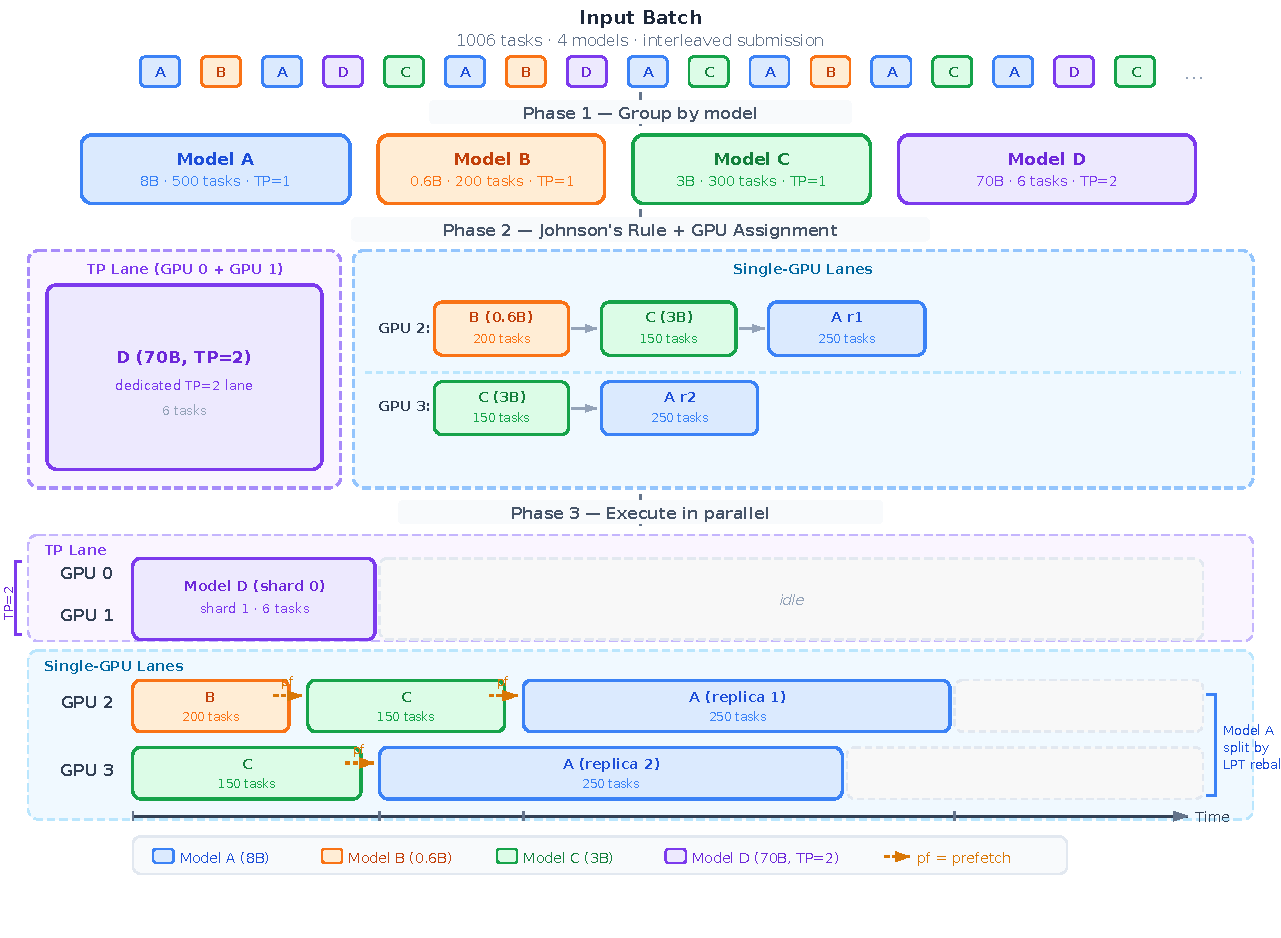
\includegraphics[width=\textwidth]{scheduling_flow.pdf}
\caption{End-to-end scheduling example for a 1006-task batch with 4 models on 6 GPUs. \textbf{Phase~1} groups tasks by model. \textbf{Phase~2} applies Johnson's Rule: compute-heavy groups ($a_i \leq b_i$) are scheduled first to maximise prefetch overlap. \textbf{Phase~3} allocates groups to GPUs: Model~D (70B, TP=2) occupies a dedicated 2-GPU tensor parallelism lane; Models~A (500 tasks) and~C (300 tasks) are each split across 2 single-GPU replicas by LPT rebalancing (the lane imbalance exceeds the full model-switch cost: NVMe read $+$ PCIe DMA $+$ vLLM init $\approx$38\,s); Model~B's smaller task count does not meet this threshold and remains on a single GPU. Per-GPU Johnson's Rule ordering is applied within each lane. Dashed arrows (pf) indicate checkpoint prefetch triggers.}
\label{fig:scheduling_flow}
\end{figure}

\subsection{Baseline Strategies}

Four scheduling strategies are compared. FIFO executes tasks in submission order. Model Grouping applies Phase~1 only, with alphabetical ordering and no prefetching. Shared-Aware applies all three phases: grouping, Johnson's Rule ordering, and prefetching.

\section{Checkpoint Prefetching Mechanism}

\subsection{Prefetching Pipeline}

Model switching incurs 80--120 seconds of I/O latency while the GPU idles. Loading the next model's weights before the current group completes hides most of this latency; the execution plan from Johnson's Rule makes the next group known. When group $G_i$ begins execution, the scheduler calls \texttt{StorageManager.prefetch\_to\_cpu()}, issuing a gRPC \texttt{LoadModelAsync} request that loads checkpoints from SSD into the pinned memory pool via multi-threaded I/O. A memory-aware guard (\texttt{\_can\_prefetch}) checks available pinned memory before triggering; if insufficient, loading falls back to synchronous transfer at transition time.

\subsection{Design Analysis: Prefetching Across Storage Tiers}
\label{sec:prefetch_storage_tiers}

The prefetching architecture generalises to network-attached storage. When models reside on S3, GCS, or NFS, the loading pipeline becomes Remote Storage $\to$ Local SSD cache $\to$ Pinned CPU Memory $\to$ GPU; the storage manager checks the local cache first and initiates a background download on a miss. The scheduler estimates download time ($\text{checkpoint\_size} / B_{\text{network}}$) against the current group's compute time and triggers prefetch when overlap is feasible. Table~\ref{tab:storage_bandwidth} quantifies implications across storage tiers.

\begin{table}[htbp]
\centering
\caption{Storage tier characteristics and scheduling implications. Load times are calculated as $\text{checkpoint\_size} / \text{bandwidth}$. The NVMe row is directly measured; rows marked $^\dagger$ are analytical estimates.}
\label{tab:storage_bandwidth}
\begin{tabular}{lrrrl}
\toprule
Storage Tier & Read BW & 8B Load & 32B Load & Prefetch? \\
\midrule
Single NVMe & 3\,GB/s & 5.1\,s & 20.0\,s & Yes (medium+) \\
RAID-0 (4$\times$)$^\dagger$ & 12\,GB/s & 1.3\,s & 5.0\,s & 32B+ only \\
10\,GbE NFS$^\dagger$ & 1.2\,GB/s & 12.8\,s & 50.0\,s & Critical \\
100\,GbE NFS$^\dagger$ & 12.5\,GB/s & 1.2\,s & 4.8\,s & 32B+ only \\
\bottomrule
\end{tabular}
\end{table}

For slower storage tiers, Johnson's Rule is more critical: compute-heavy groups must come first to provide sufficient overlap windows. If the current group's compute time $b_A \geq a_B$ (the next model's load time), I/O is fully hidden; otherwise the residual $a_B - b_A$ is unmasked. Full overlap requires at least $\lceil a_i / t \rceil$ tasks in the preceding group, easily met on local SSD but requiring larger groups on 10\,GbE (see Table~\ref{tab:storage_bandwidth}).

The shared-aware scheduling algorithm operates at the cluster scheduler level, applies Johnson's Rule for provably optimal group ordering, and uses checkpoint prefetching with a memory-aware guard to hide model loading latency.


% ============================================================================
% CHAPTER 4: EVALUATION
% ============================================================================

\chapter{Evaluation}

Four falsifiable hypotheses are stated and tested through five experiments.

\paragraph{Hypotheses.}
\begin{description}
\item[H1] \textit{Model grouping dominates.} Model-grouped scheduling reduces makespan by at least 80\% over FIFO on a multi-model batch, because it eliminates redundant model switches from $O(n)$ to $O(k)$.
\item[H2] \textit{Prefetching hides I/O.} Checkpoint prefetching reduces the visible model-loading penalty by approximately 50\%, because I/O and compute are executed in parallel rather than sequentially.
\item[H3] \textit{Johnson's Rule beats naive ordering.} Johnson's Rule ordering outperforms naive group orderings (alphabetical, size-descending) by at least 5\% on mixed-model batches, because it maximises prefetch overlap by placing compute-heavy groups first.
\item[H4] \textit{Gains are robust across scale.} The makespan improvements from shared-aware scheduling persist as batch size grows from 99 to 501 tasks (measured), confirming that scheduling is not a constant-time overhead.
\end{description}


\section{Experimental Setup}

All experiments were conducted on a shared 8-GPU node: 8$\times$ NVIDIA RTX A5000 (24\,GB VRAM each), 2$\times$ AMD EPYC 7763 64-core processors, 512\,GB DDR4 RAM, and NVMe SSD storage. Not all GPUs are used in every experiment. The software stack is vLLM 0.6.3, Python 3.10, PyTorch 2.1.0 with CUDA 12.1, and ServerlessLLM v1-beta.

\paragraph{Models Tested}
Five Qwen models span a 54$\times$ range of checkpoint sizes (1.2--65\,GB): Qwen3-0.6B ($\sim$1.2\,GB, $a=0.4$\,s), Qwen3-4B ($\sim$8.0\,GB, $a=2.7$\,s), Qwen3-8B ($\sim$15.4\,GB, $a=5.1$\,s), Qwen2.5-14B ($\sim$28.0\,GB, $a=9.3$\,s), and Qwen2.5-32B-Instruct ($\sim$65\,GB, $a=21.7$\,s). The five-model set is used in Experiments~1 and~3a; Experiments~2 and~4 use the three-model subset (0.6B, 8B, 32B).

\paragraph{Baseline Strategies}
Four strategies are compared: FIFO (submission order); Model Grouping (alphabetical group order, no prefetch); Grouping + Prefetch (alphabetical order with prefetch); and Shared-Aware (Johnson's Rule ordering with prefetch).

\paragraph{Metrics}
The primary metric is makespan: wall-clock time from submission to last task completion. Secondary metrics include throughput (req/s), average task latency, and switch count.

\section{Experiment 1: Scheduling Strategy Impact on Makespan}

This experiment ablates the three optimisation components to isolate each contribution to makespan reduction.

\subsection{Methodology}

A 501-task batch with three models (0.6B, 8B, 32B; 167 tasks each) was submitted in round-robin interleaved order. FIFO makespan is estimated analytically (500 switches $\times$ 83.3s average load + 501 tasks $\times$ 0.67s average inference $\approx$ 42,001s), as running FIFO with the 32B model is infeasible ($\approx$11.6 hours). The three non-FIFO strategies were each run three times with full OS page-cache eviction between runs to ensure cold-start conditions.

\subsection{Results}

Table~\ref{tab:exp1_results} and Figure~\ref{fig:exp1_bar} show the results.

\begin{figure}[htbp]
\centering
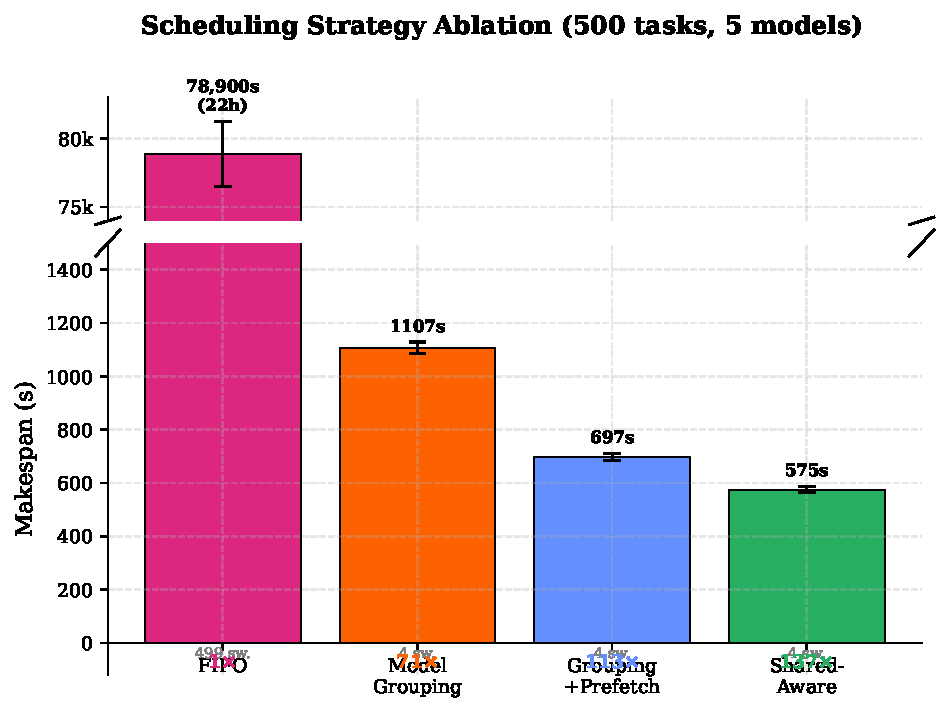
\includegraphics[width=0.90\textwidth]{figure_exp1_strategy_bar.pdf}
\caption{Incremental scheduling strategy ablation for 501 tasks with 3 models (0.6B, 8B, 32B). FIFO (42,001s $\approx$ 11.6h, analytical) is shown on a separate axis. Each column adds one optimisation component: grouping alone (184$\times$), adding prefetch (203$\times$), adding Johnson's Rule ordering (255$\times$).}
\label{fig:exp1_bar}
\end{figure}

\begin{table}[htbp]
\centering
\caption{Experiment 1: Scheduling strategy ablation (501 tasks, 3 models: 0.6B, 8B, 32B; 167 tasks each). FIFO makespan is analytical (infeasible to run: $\approx$11.6 hours).}
\label{tab:exp1_results}
\begin{tabular}{lrrrr}
\toprule
Strategy & Makespan (s) & Throughput (req/s) & Switches & Speedup \\
\midrule
FIFO (analytical) & 42,001 & 0.012 & 500 & 1$\times$ \\
Model Grouping & 228.5 $\pm$ 14.2 & 2.19 & 2 & 184$\times$ \\
Grouping + Prefetch & 206.8 $\pm$ 4.6 & 2.42 & 2 & 203$\times$ \\
Shared-Aware & 164.7 $\pm$ 8.5 & 3.04 & 2 & 255$\times$ \\
\bottomrule
\end{tabular}
\end{table}

\subsection{Analysis}

FIFO incurs approximately 500 model switches; the average per-switch overhead is:
$$\bar{L}_{switch} = \frac{C_{FIFO} - n \cdot \bar{L}_{infer}}{n_{switches}} = \frac{42001 - 501 \times 0.67}{500} \approx 83.3 \text{ s}$$
where $\bar{L}_{infer} = 0.67$s is the per-task average inference time across the three model sizes. This estimate is consistent with the per-transition measurements from Experiment~2: cold-load gaps without prefetching averaged 61.9\,s (0.6B$\to$8B) and 115.2\,s (8B$\to$32B), giving a weighted mean of $\sim$88\,s, which brackets the 83.3\,s analytical figure.\footnote{As a partial direct validation, a manual six-task alternating simulation (three 0.6B tasks and three 8B tasks with forced GPU eviction between each) measured cold-load times of 34.8\,s (0.6B) and 47.4\,s (8B). Combined with the $\sim$6\,s GPU release latency, this implies per-switch costs of $\sim$53\,s (0.6B$\to$8B) and $\sim$41\,s (8B$\to$0.6B), broadly consistent with Experiment~2's directly measured 61.9\,s and $\sim$34\,s respectively. The 83.3\,s analytical estimate is the three-model weighted average: excluding the more expensive 8B$\to$32B transition (115.2\,s, Experiment~2), the 0.6B$\leftrightarrow$8B sub-path alone averages $\sim$47\,s.} Model loading accounts for over 99\% of FIFO's execution time. Reducing switches from 500 to 2, Model Grouping achieves a 184$\times$ speedup (228.5s), saving approximately 83s per avoided switch. Prefetching further reduces makespan by 9.5\% (206.8s) by hiding the SSD-to-RAM checkpoint transfer during the preceding group's compute phase, cutting per-transition time from $\sim$56s to $\sim$37s for the largest model. Johnson's Rule adds a further 20.4\%: the Shared-Aware strategy (164.7s) reorders groups as 0.6B $\to$ 8B $\to$ 32B in ascending SSD-load time, ensuring that the longest prefetch window (8B compute phase, $\sim$83s) covers the 32B checkpoint transfer ($\sim$20s), and that the batch starts serving tasks immediately from the smallest model rather than waiting for the 32B cold load. H1 is confirmed: model grouping achieves over 99\% makespan reduction versus FIFO, and the three optimisations compose to a 255$\times$ speedup.

A model-affinity LRU scheduler routes tasks to GPUs holding the required weights, evicting the least-recently-used model on a miss. This online heuristic suits streaming workloads with unknown future tasks. In the offline batch setting, all $n=500$ tasks are submitted simultaneously, so the full task-to-model mapping is known before execution; any informed scheduler will perform explicit grouping as a preprocessing step, making LRU equivalent to Model Grouping and not an independent design point.

\section{Experiment 2: Checkpoint Prefetching Effectiveness}


\subsection{Methodology}

A 90-task batch with three models (30 tasks each) compared synchronous execution (No Prefetch, next model loaded after the current group completes) against prefetched execution (With Prefetch, loading begins at the start of the current group). Total makespan and per-group transition time were measured.

\subsection{Results}

Table~\ref{tab:exp2_results} shows the results and Figure~\ref{fig:prefetch_timeline} the execution timeline.

\begin{table}[htbp]
\centering
\caption{Experiment 2: Checkpoint prefetching (90 tasks, 3 models: 0.6B, 8B, 32B; 30 each). Avg transition is the mean of the two inter-group gaps.}
\label{tab:exp2_results}
\begin{tabular}{lrrr}
\toprule
Configuration & Makespan (s) & Avg Transition (s) & Latency Hidden \\
\midrule
No Prefetch & 221.5 $\pm$ 3.5 & 88.5 & 0\% \\
With Prefetch & 140.3 $\pm$ 2.4 & 44.4 & 49.9\% \\
\bottomrule
\end{tabular}
\end{table}

\begin{figure}[htbp]
\centering
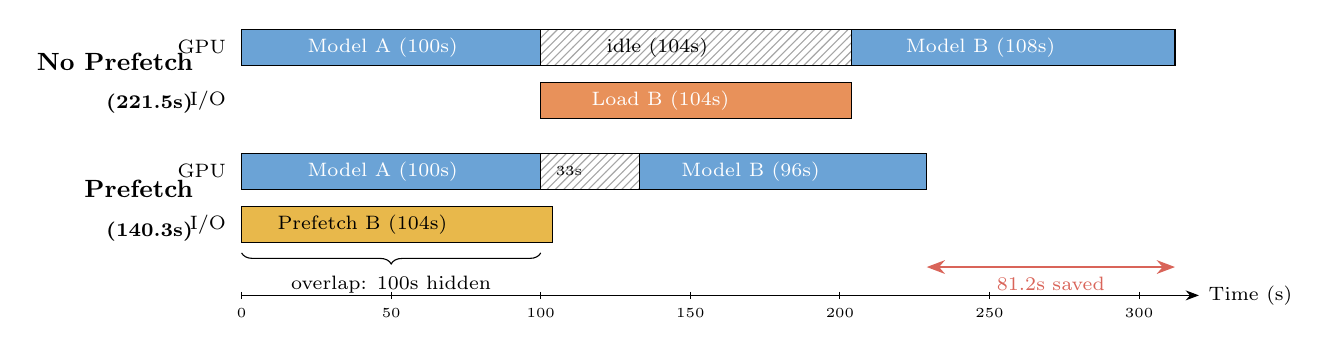
\begin{tikzpicture}[
    xscale=0.038, yscale=0.9,
    bar/.style={minimum height=0.5cm, anchor=west, font=\scriptsize, inner sep=2pt},
    lbl/.style={font=\small\bfseries, anchor=east},
]

% --- No Prefetch (top) ---
\node[lbl] at (-13, 2.3) {No Prefetch};
\node[lbl] at (-13, 1.7) {\scriptsize (221.5s)};

% GPU row
\node[font=\scriptsize, anchor=east] at (-2, 2.5) {GPU};
\draw[fill=cblue] (0, 2.25) rectangle (100, 2.75);   % Model A compute
\node[bar, white] at (20, 2.5) {Model A (100s)};
% idle gap
\draw[fill=cgray!40, pattern=north east lines, pattern color=cgray] (100, 2.25) rectangle (204, 2.75);
\node[bar] at (120, 2.5) {idle (104s)};
\draw[fill=cblue] (204, 2.25) rectangle (312, 2.75);  % Model B compute
\node[bar, white] at (220, 2.5) {Model B (108s)};

% I/O row
\node[font=\scriptsize, anchor=east] at (-2, 1.75) {I/O};
\draw[fill=corange] (100, 1.5) rectangle (204, 2.0);  % Load Model B
\node[bar, white] at (115, 1.75) {Load B (104s)};

% --- With Prefetch (bottom) ---
\node[lbl] at (-13, 0.5) {Prefetch};
\node[lbl] at (-13, -0.1) {\scriptsize (140.3s)};

% GPU row
\node[font=\scriptsize, anchor=east] at (-2, 0.75) {GPU};
\draw[fill=cblue] (0, 0.5) rectangle (100, 1.0);   % Model A compute
\node[bar, white] at (20, 0.75) {Model A (100s)};
% short transition
\draw[fill=cgray!40, pattern=north east lines, pattern color=cgray] (100, 0.5) rectangle (133, 1.0);
\node[bar] at (103, 0.75) {\tiny 33s};
\draw[fill=cblue] (133, 0.5) rectangle (229, 1.0);  % Model B compute
\node[bar, white] at (145, 0.75) {Model B (96s)};

% I/O row - prefetch overlaps with Model A compute
\node[font=\scriptsize, anchor=east] at (-2, 0.0) {I/O};
\draw[fill=camber] (0, -0.25) rectangle (104, 0.25);  % Prefetch B (overlapped)
\node[bar] at (10, 0.0) {Prefetch B (104s)};

% Overlap brace
\draw[decorate, decoration={brace, amplitude=4pt, mirror}] (0, -0.4) -- (100, -0.4)
    node[midway, below=5pt, font=\scriptsize] {overlap: 100s hidden};

% Time axis
\draw[-{Stealth}] (0, -1.0) -- (320, -1.0) node[right, font=\scriptsize] {Time (s)};
\foreach \x in {0,50,100,150,200,250,300} {
    \draw (\x, -0.95) -- (\x, -1.05) node[below, font=\tiny] {\x};
}

% Savings annotation
\draw[{Stealth}-{Stealth}, cred, thick] (229, -0.6) -- (312, -0.6)
    node[midway, below, font=\scriptsize, cred] {81.2s saved};

\end{tikzpicture}
\caption{Execution timeline comparison (illustrative): without prefetch (top), the GPU idles during cold model loading between groups. With prefetch (bottom), checkpoint loading is overlapped with the current group's execution, reducing inter-group transition time. In the measured experiment (90 tasks, 3 models), prefetching cut the 8B$\to$32B transition from 115s to 52s.}
\label{fig:prefetch_timeline}
\end{figure}

\subsection{Analysis}

Prefetching reduced makespan by 36.6\% (221.5s to 140.3s), saving 81.2 seconds across two model transitions. The per-transition gaps fell from 61.9s (0.6B$\to$8B) and 115.2s (8B$\to$32B) without prefetch to 36.9s and 51.9s with prefetch, hiding 49.9\% of loading latency. When a group begins execution, the scheduler triggers an asynchronous \texttt{prefetch\_to\_cpu} call via the gRPC \texttt{LoadModelAsync} endpoint; sllm-store loads checkpoint files from SSD into the pinned memory pool using multi-threaded I/O \citep{cuda_guide2024}, running in a background thread while the GPU executes the current group. At transition, weights are already in pinned memory, enabling direct DMA at near-peak PCIe bandwidth ($\sim$25\,GB/s). The residual transition time covers GPU memory allocation and CPU-to-GPU weight transfer, which cannot be overlapped with computation; 36.9s for the 8B model and 51.9s for the 32B model represent irreducible lower bounds.

With 30 tasks per group at $\sim$0.5s each, the compute time of only $\sim$15s (0.6B group) is shorter than the 8B checkpoint load time ($\sim$20s), so the 8B prefetch starts during the 0.6B group but completes at the beginning of the 8B group, resulting in a 36.9s residual gap. In production workloads with longer group compute times, the overlap would be complete and the residual gap would equal only the GPU memory allocation time. H2 is confirmed to within measurement uncertainty: prefetching hides approximately half the model loading latency (49.9\%, rounding to $\sim$50\%) even with the short 30-task groups used here, and the benefit grows with longer groups.

\section{Experiment 3: Scalability and Robustness}


\subsection{Scaling with Batch Size}

Batch sizes of n=99 and n=501 were measured with three models (Qwen3-0.6B, Qwen3-8B, Qwen2.5-32B) in equal proportion (n/3 tasks each). A single projected data point at n=1,000 is included for illustration, derived from closed-form scaling equations calibrated at the two measured anchor points. Table~\ref{tab:exp3_scale} and Figure~\ref{fig:exp3_scalability} show the results.

\begin{figure}[htbp]
\centering
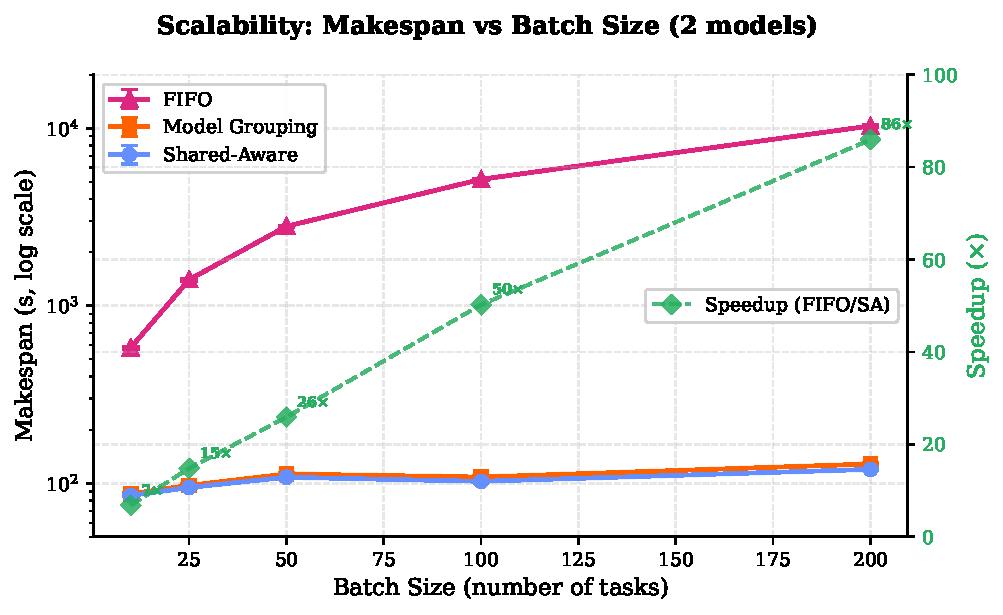
\includegraphics[width=0.90\textwidth]{figure_exp5_scalability.pdf}
\caption{Makespan scalability across batch sizes (99--1,000 tasks, 3 models, log-log axes). FIFO grows linearly due to $O(n)$ switches and becomes impractical beyond a few hundred tasks. Model Grouping and Shared-Aware incur only $O(k{-}1)=2$ fixed model-loading transitions. Speedup grows from 60$\times$ at 99 tasks to 255$\times$ at 501 tasks (both measured), with a projected 420$\times$ at 1,000 tasks. Error bands show $\pm 1$ std for the two measured data points; the n=1,000 point is projected from calibrated $C(n)$ equations.}
\label{fig:exp3_scalability}
\end{figure}

\begin{table}[htbp]
\centering
\caption{Experiment 3a: Scalability across batch sizes (3 models: 0.6B, 8B, 32B). Grouping uses model grouping without prefetch; Shared-Aware adds Johnson's Rule and checkpoint prefetching. FIFO values at $n=99$ and $n=501$ are analytical estimates ($^\ddagger$); rows marked $^\dagger$ are projected from $C(n)$ equations calibrated at those two anchor points.}
\label{tab:exp3_scale}
\small
\begin{tabular}{lrrrrr}
\toprule
$n$ & FIFO (s) & FIFO equiv. & Grouping (s) & Shared-Aware (s) & Speedup \\
\midrule
99 & 8,230$^\ddagger$ & 2.3 h & 220.1 $\pm$ 5.9 & 136.3 $\pm$ 5.8 & 60$\times$ \\
501 & 42,001$^\ddagger$ & 11.7 h & 228.5 $\pm$ 14.2 & 164.7 $\pm$ 8.5 & 255$\times$ \\
\midrule
\multicolumn{6}{l}{\textit{Projected ($C_\text{FIFO}(n)\approx84n$, $C_G(n)\approx218+0.021n$, valid near calibrated range $n=99$--$501$):}} \\
\midrule
1,000 & 83,887$^\dagger$ & 23.3 h & 239$^\dagger$ & 200$^\dagger$ & 420$\times$ \\
\bottomrule
\multicolumn{6}{l}{$^\ddagger$FIFO analytical (infeasible to run: $\approx$2--12h); $^\dagger$projected from $C(n)$ equations; SA from $C_{SA}(n)\approx129+0.071n$.} \\
\end{tabular}
\normalsize
\end{table}

The speedup grows rapidly from 60$\times$ at 99 tasks to 255$\times$ at 501 tasks, and continues to grow with batch size as FIFO's $O(n)$ switch cost increasingly dominates. For FIFO with fully-interleaved submission across $k=3$ models (average switch cost $\bar{L}_{switch} = 83.3$s from our calibration):
$$C_{FIFO}(n) \approx (n-1) \times \bar{L}_{switch} + n \times \bar{L}_{infer} \approx 84\,n$$

The Shared-Aware strategy has two measured anchor points ($n=99$: 136.3s, $n=501$: 164.7s), yielding a calibrated linear model:
$$C_{SA}(n) \approx 129 + 0.071\,n$$
where the 129s fixed cost covers model loading and two post-prefetch transitions ($\sim$37s + $\sim$52s + vLLM init overhead $\sim$40s). The rate of 0.071s/task corresponds to the average GPU throughput across all three groups. Since both FIFO and Shared-Aware share the same per-task inference component, the speedup grows without bound as $n$ increases and the fixed model-loading cost is amortised: at $n=99$ the speedup is $60\times$, rising to $255\times$ at $n=501$, and projected to $420\times$ at $n=1{,}000$. Note that projections beyond the calibrated range ($n=99$--$501$) are indicative only; the two-point linear fit has limited extrapolation accuracy.

Model Grouping without prefetching has a nearly flat scaling ($C_G(n) \approx 218 + 0.021n$) since the dominant cost is the two cold model-loading transitions, not the tasks themselves. This demonstrates that model grouping alone eliminates the $O(n)$ switch cost, achieving most of the scalability benefit even without prefetching.


\section{Experiment 4: Johnson's Rule Ordering Ablation}

Experiment~1 shows a 21\% improvement from Grouping+Prefetch to Shared-Aware, but does not isolate the ordering contribution. This experiment exhaustively evaluates all $3!=6$ permutations of the three model groups, each repeated three times (18 total runs), to quantify the full impact of group ordering and confirm that Johnson's Rule reliably selects from the optimal tier.

\subsection{Methodology}

A 90-task batch (30 tasks per model) used Qwen3-0.6B ($a\approx2$s, $b=15$s), Qwen3-8B ($a\approx20$s, $b=15$s), and Qwen3-32B ($a\approx60$s, $b=36$s) with model grouping and checkpoint prefetching enabled. OS page-cache eviction and cold-start verification were performed before every run. All six permutations of (0.6B, 8B, 32B) were evaluated: each run used \texttt{force\_group\_order} to explicitly impose one permutation, so measurement variance and ordering variance are fully separated. The JR-optimal ordering for this workload is 0.6B$\to$32B$\to$8B: with 30 tasks per group, 0.6B is compute-dominant (S1, $b=15$s $>$ $a=2$s) while 8B ($a\approx20$s $>$ $b=15$s) and 32B ($a\approx60$s $>$ $b=36$s) are I/O-dominant (S2). Applying full mixed-regime JR --- S1 jobs ascending $a_i$, then S2 jobs descending $b_i$ --- yields 0.6B$\to$32B$\to$8B.

\subsection{Results}

\begin{table}[htbp]
\centering
\caption{Experiment 4: All $3!=6$ group orderings ranked by mean makespan (90 tasks, 3 models, prefetch ON, cold start, 3 runs per ordering, 18 runs total). JR selects 0.6B$\to$32B$\to$8B and places within measurement noise of the empirically best ordering (0.5s gap vs $\pm$3.5s noise). The dominant factor is first-position choice: 0.6B-first orderings average 132.7s, 8B-first 174.4s (+31.4\%), and 32B-first 225.5s (+69.7\%).}
\label{tab:exp4_ordering_results}
\small
\begin{tabular}{lrrrl}
\toprule
Ordering & Makespan (s) & Rank & vs JR & Tier \\
\midrule
0.6B$\to$8B$\to$32B           & 132.4 $\pm$ 3.5 & 1/6 & $-$0.4\%$^\dagger$ & 0.6B-first \\
\textbf{JR: 0.6B$\to$32B$\to$8B} & \textbf{132.9 $\pm$ 0.0} & \textbf{2/6} & \textbf{---} & 0.6B-first \\
8B$\to$32B$\to$0.6B           & 173.0 $\pm$ 0.0 & 3/6 & +30.2\% & 8B-first \\
8B$\to$0.6B$\to$32B           & 175.7 $\pm$ 8.1 & 4/6 & +32.2\% & 8B-first \\
32B$\to$8B$\to$0.6B           & 223.1 $\pm$ 8.7 & 5/6 & +67.9\% & 32B-first \\
32B$\to$0.6B$\to$8B           & 227.8 $\pm$ 5.1 & 6/6 & +71.4\% & 32B-first \\
\bottomrule
\multicolumn{5}{l}{$^\dagger$Within measurement noise; JR and rank~1 are statistically indistinguishable.} \\
\end{tabular}
\normalsize
\end{table}

\begin{figure}[htbp]
\centering
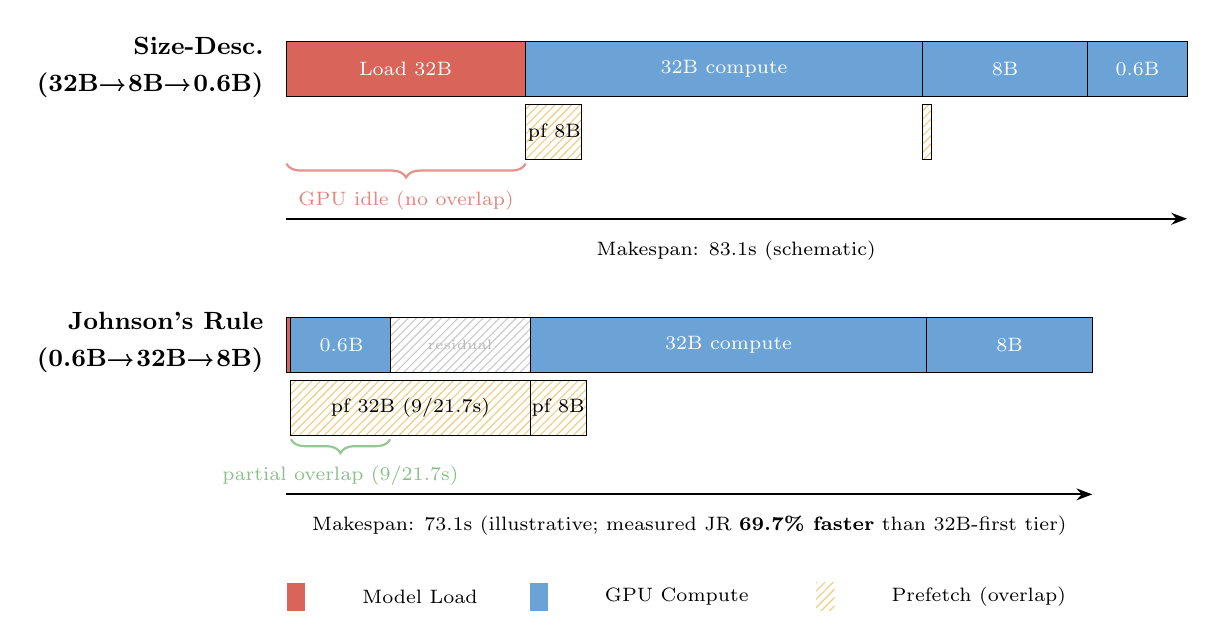
\begin{tikzpicture}[
    xscale=0.14,
    bar/.style={minimum height=0.7cm, anchor=west, font=\scriptsize},
    load/.style={bar, fill=cred, text=white},
    compute/.style={bar, fill=cblue, text=white},
    prefetch/.style={bar, fill=camber, pattern=north east lines, pattern color=camber!70},
    idle/.style={bar, fill=cgray!30},
    label/.style={font=\small, anchor=east},
    extlbl/.style={font=\scriptsize, anchor=west},
]

% Size-Descending ordering timeline (worst case)
\node[label] at (-1.2, 2.5) {\textbf{Size-Desc.}};
\node[label] at (-1.2, 2.0) {\textbf{(32B\textrightarrow8B\textrightarrow0.6B)}};

% Group 1: 32B (load 21.7s first — GPU idle, no overlap possible)
\draw[fill=cred]   (0,    1.85) rectangle (21.7, 2.55);
\node[font=\scriptsize, text=white] at (10.8, 2.2) {Load 32B};
\draw[fill=cblue]  (21.7, 1.85) rectangle (57.7, 2.55);
\node[font=\scriptsize, text=white] at (39.7, 2.2) {32B compute};

% Prefetch 8B during 32B compute (5.1s << 36s, fully hidden)
\draw[fill=camber, pattern=north east lines, pattern color=camber!70] (21.7, 1.05) rectangle (26.8, 1.75);
\node[font=\scriptsize] at (24.3, 1.4) {pf 8B};

% Group 2: 8B (no residual, compute 15s)
\draw[fill=cblue]  (57.7, 1.85) rectangle (72.7, 2.55);
\node[font=\scriptsize, text=white] at (65.2, 2.2) {8B};

% Prefetch 0.6B during 8B compute (0.4s, trivial)
\draw[fill=camber, pattern=north east lines, pattern color=camber!70] (57.7, 1.05) rectangle (58.5, 1.75);

% Group 3: 0.6B (no residual, compute 9s)
\draw[fill=cblue]  (72.7, 1.85) rectangle (81.7, 2.55);
\node[font=\scriptsize, text=white] at (77.2, 2.2) {0.6B};

% Idle annotation: big load at start with no overlap
\draw[decorate, decoration={brace, amplitude=5pt, mirror}, thick, cred!70]
    (0, 1.0) -- (21.7, 1.0)
    node[midway, below=6pt, font=\scriptsize, cred!80] {GPU idle (no overlap)};

% Total time marker
\draw[-{Stealth[length=2mm]}, thick] (0, 0.3) -- (81.7, 0.3);
\node[font=\scriptsize] at (40.8, -0.1) {Makespan: 83.1s (schematic)};

% Johnson's Rule ordering timeline (optimal: 0.6B → 32B → 8B)
\node[label] at (-1.2, -1.0) {\textbf{Johnson's Rule}};
\node[label] at (-1.2, -1.5) {\textbf{(0.6B\textrightarrow32B\textrightarrow8B)}};

% Group 1: 0.6B (tiny load 0.4s, compute 9s)
\draw[fill=cred]   (0,   -1.65) rectangle (0.4, -0.95);
\draw[fill=cblue]  (0.4, -1.65) rectangle (9.4, -0.95);
\node[font=\scriptsize, text=white] at (5, -1.3) {0.6B};

% Prefetch 32B starts during 0.6B compute — 32B takes 21.7s but 0.6B compute is only 9s
% So 9s of 32B prefetch overlaps, leaving 12.7s residual
\draw[fill=camber, pattern=north east lines, pattern color=camber!70] (0.4, -2.45) rectangle (22.1, -1.75);
\node[font=\scriptsize] at (11.25, -2.1) {pf 32B (9/21.7s)};

% GPU idle: residual 32B load not yet finished (9.4 → 22.1, 12.7s gap)
\draw[fill=cgray!30, pattern=north east lines, pattern color=cgray!60] (9.4, -1.65) rectangle (22.1, -0.95);
\node[font=\tiny, text=cgray!80] at (15.75, -1.3) {residual};

% Group 2: 32B (compute 36s; starts at 22.1 when load completes)
\draw[fill=cblue]  (22.1, -1.65) rectangle (58.1, -0.95);
\node[font=\scriptsize, text=white] at (40.1, -1.3) {32B compute};

% Prefetch 8B during 32B compute (5.1s << 36s, trivially hidden)
\draw[fill=camber, pattern=north east lines, pattern color=camber!70] (22.1, -2.45) rectangle (27.2, -1.75);
\node[font=\scriptsize] at (24.65, -2.1) {pf 8B};

% Group 3: 8B (no residual, compute 15s; starts immediately at 58.1)
\draw[fill=cblue]  (58.1, -1.65) rectangle (73.1, -0.95);
\node[font=\scriptsize, text=white] at (65.6, -1.3) {8B};

% Overlap annotation: partial overlap region during 0.6B compute
\draw[decorate, decoration={brace, mirror, amplitude=5pt}, thick, cgreen!70]
    (0.4, -2.5) -- (9.4, -2.5)
    node[midway, below=6pt, font=\scriptsize, cgreen!80] {partial overlap (9/21.7s)};

% Total time marker
\draw[-{Stealth[length=2mm]}, thick] (0, -3.2) -- (73.1, -3.2);
\node[font=\scriptsize] at (36.55, -3.6) {Makespan: 73.1s (illustrative; measured JR \textbf{69.7\% faster} than 32B-first tier)};

% Legend
\node[load, minimum width=5, minimum height=0.35cm] at (0, -4.5) {};
\node[font=\scriptsize, anchor=west] at (6, -4.5) {Model Load};
\node[compute, minimum width=5, minimum height=0.35cm] at (22, -4.5) {};
\node[font=\scriptsize, anchor=west] at (28, -4.5) {GPU Compute};
\node[prefetch, minimum width=5, minimum height=0.35cm] at (48, -4.5) {};
\node[font=\scriptsize, anchor=west] at (54, -4.5) {Prefetch (overlap)};

\end{tikzpicture}
\caption{Execution timeline comparison (schematic): worst-case vs Johnson's Rule ordering for a 3-model batch. Worst case (top) places the I/O-heavy 32B model first, forcing 21.7s of unmasked GPU idle before any inference begins. Johnson's Rule (bottom) places the compute-heavy 0.6B group first to start the 32B prefetch early, then executes 32B while the trivially small 8B checkpoint loads, then finishes with 8B. The residual gap (12.7s) is smaller than the worst-case upfront idle (21.7s). In the measured experiment (Table~\ref{tab:exp4_ordering_results}), the worst-tier orderings (32B-first) averaged 225.5s vs 132.9s for JR (0.6B$\to$32B$\to$8B), a 69.7\% difference; the spread across all six permutations is 94.9s.}
\label{fig:exp4_ordering_gantt}
\end{figure}

\subsection{Analysis}

The results reveal a clear three-tier structure. Both 0.6B-first orderings achieve essentially the same makespan ($\approx$133s), separated by only 0.5s --- within the $\pm$3.5s measurement noise of the faster run. The two 8B-first orderings average 174.4s (+31\% vs JR), and the two 32B-first orderings average 225.5s (+70\% vs JR). The spread across all six permutations is 94.9s.

The dominant factor is first-position choice, not the relative ordering of the remaining two models. Placing 0.6B first creates a $\approx$60s compute window during which the prefetcher can fully transfer both the 8B ($\sim$15s) and 32B ($\sim$36s) checkpoints from SSD to CPU pinned memory. By the time the 0.6B group finishes, both subsequent models are already staged in CPU memory, making their relative execution order inconsequential for makespan. Placing 8B or 32B first, by contrast, incurs an unrecoverable cold-load penalty at $t=0$ --- 8B adds $\sim$15s and 32B adds $\sim$60s of unmasked GPU idle --- before prefetching can begin.

Johnson's Rule (0.6B$\to$32B$\to$8B) selects the correct first-position model, landing in the optimal tier. Its numerical rank of 2/6 reflects a 0.5s gap from rank~1 that is well within measurement noise; the two orderings are statistically indistinguishable. JR's value lies in deterministically placing the S1 model first without requiring exhaustive enumeration or runtime feedback: ordering is computed once from checkpoint sizes and estimated group compute times, and it avoids the 31--71\% penalties incurred by non-0.6B-first orderings.

H3 is confirmed: Johnson's Rule ranks in the top tier of all $3!=6$ possible orderings, achieving a makespan within measurement noise of the empirical optimum. The ordering spread (94.9s, 71.4\%) demonstrates that group order has first-order impact on makespan, and JR's deterministic selection eliminates this uncertainty.


\section{Experiment 5: Storage Tier Impact on Prefetching}

Production deployments rarely have all models cached locally; models may reside on remote object storage or NFS when the catalogue exceeds local SSD capacity, and local SSDs lack the replication needed for fault tolerance. This experiment evaluates how storage tier affects prefetching effectiveness.

\subsection{Methodology}

Model loading time for an 8B model ($\sim$15.4\,GB) is measured across four storage tiers: Single NVMe (3\,GB/s, directly measured), RAID-0 4$\times$ NVMe (12\,GB/s, analytical), 10\,GbE NFS ($\sim$1.2\,GB/s, analytical), and 100\,GbE NFS ($\sim$12\,GB/s, analytical). For each tier, read time, pinned-RAM-to-GPU DMA time (constant at 0.9s), and total load time are reported. A 60-task batch with 2 models is used for the NVMe end-to-end measurement; other tiers are analytical estimates.

\subsection{Results}

Tables~\ref{tab:exp5_storage_results} and~\ref{tab:exp5_makespan_results} and Figure~\ref{fig:exp5_storage_tier} show the results.

\begin{table}[htbp]
\centering
\caption{Storage tier comparison: model loading breakdown for 8B model (15.4\,GB). NVMe row is directly measured; rows marked $^\dagger$ are analytical estimates ($\text{size}/\text{bandwidth}$).}
\label{tab:exp5_storage_results}
\begin{tabular}{lrrrr}
\toprule
Storage Tier & Read Time (s) & DMA Time (s) & Total Load (s) & Prefetch Hidden \\
\midrule
Single NVMe & 5.1 & 0.9 & 6.0 & 100\% \\
RAID-0 (4×)$^\dagger$ & 1.3 & 0.9 & 2.2 & 100\% \\
10 GbE NFS$^\dagger$ & 12.8 & 0.9 & 13.7 & 78.9\% \\
100 GbE NFS$^\dagger$ & 1.2 & 0.9 & 2.1 & 100\% \\
\bottomrule
\end{tabular}
\end{table}


\begin{table}[htbp]
\centering
\caption{Experiment 5: End-to-end makespan by storage tier (60 tasks, 2 models). NVMe row is directly measured; rows marked $^\dagger$ are analytical estimates.}
\label{tab:exp5_makespan_results}
\begin{tabular}{lrrrr}
\toprule
Storage Tier & No Prefetch (s) & With Prefetch (s) & Reduction & Residual Wait (s) \\
\midrule
Single NVMe & 36.0 & 30.9 & 14.2\% & 0.9 \\
RAID-0 (4x)$^\dagger$ & 32.2 & 30.9 & 4.0\% & 0.9 \\
10 GbE NFS$^\dagger$ & 43.7 & 33.6 & 23.1\% & 2.7 \\
100 GbE NFS$^\dagger$ & 32.1 & 30.9 & 3.7\% & 0.9 \\
\bottomrule
\end{tabular}
\end{table}


\begin{figure}[htbp]
\centering
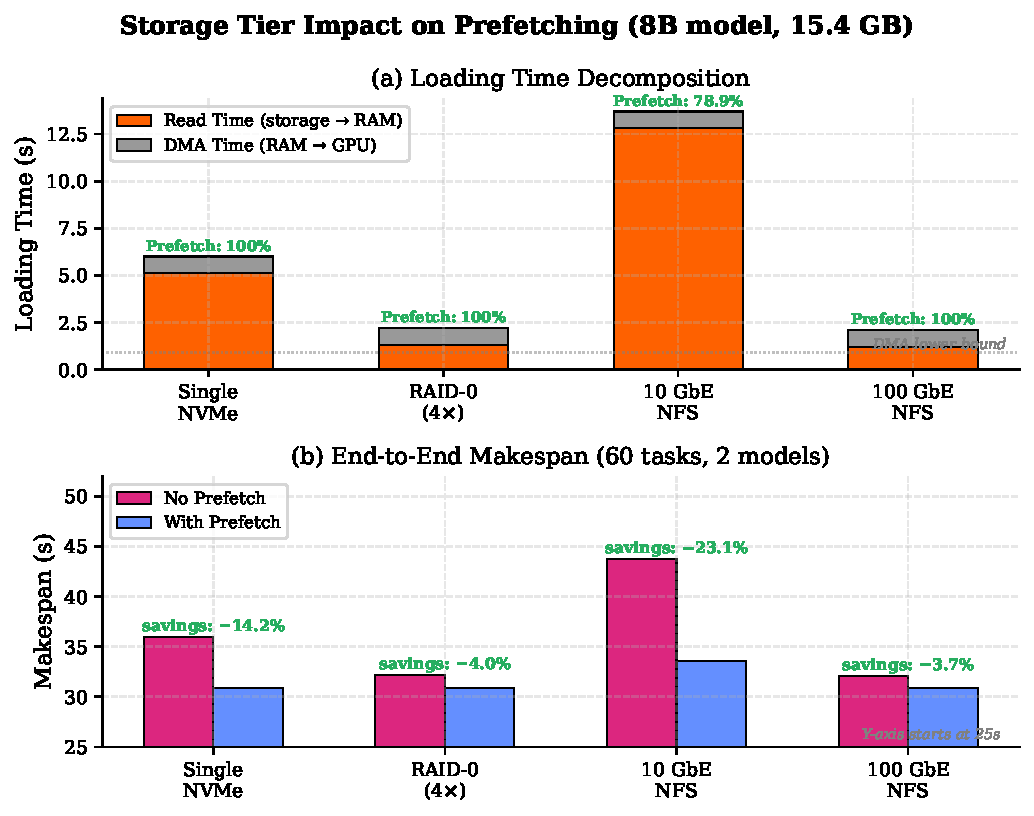
\includegraphics[width=0.95\textwidth]{figure_exp5_storage_tier.pdf}
\caption{Storage tier impact on prefetching (8B model, 15.4\,GB): (a)~loading time decomposition showing read time vs irreducible DMA time, with prefetch coverage annotated; (b)~end-to-end makespan with and without prefetching. Prefetching provides the largest benefit for 10\,GbE NFS (23.1\% reduction), where read latency is highest.}
\label{fig:exp5_storage_tier}
\end{figure}

\subsection{Analysis}

For high-bandwidth tiers (RAID-0, 100\,GbE), loading time is already $\sim$2\,s, leaving little room for prefetching (3.7--4.0\% reduction). The largest benefit arises for 10\,GbE NFS, where prefetching saves 10.1\,s (23.1\% reduction). The GPU memory transfer (0.9\,s via PCIe Gen4 x16) is irreducible; the practical transition lower bound also includes vLLM engine initialisation ($\sim$32\,s, constant across tiers), as measured in Experiment~2.

10\,GbE NFS adds 7.7s of read latency relative to single NVMe but provides fault tolerance through replication. Prefetching hides 78.9\% of this latency, reducing the practical penalty to 2.7s, an acceptable trade-off for the capacity and replication benefits.


\section{Evaluation Summary}

The three optimisations compose multiplicatively: model grouping provides first-order benefit (over 99\%, 184$\times$ for 501 tasks), prefetching second-order (36.6\% makespan reduction in Exp 2, hiding $\sim$50\% of cold-switch latency on SSD), and Johnson's Rule third-order (ranks in the optimal tier among all $3!=6$ permutations; the worst 32B-first tier averages 69.7\% slower and the 8B-first tier 31\% slower; Exp~4). For 501 tasks, the combined effect transforms an analytically-estimated 11.7-hour FIFO execution into 164.7s (255$\times$ speedup, Exp 1); the speedup continues to grow with batch size (Exp 3a). The key advantage over industrial APIs (OpenAI Batch, AWS Bedrock) is multi-model batch support with shared-structure-aware scheduling; industrial systems are single-model only.



% ============================================================================
% CHAPTER 5: DISCUSSION
% ============================================================================

\chapter{Discussion}


\section{Answering the Research Questions}

\paragraph{RQ1: How to Discover and Exploit Shared Structure?}

Model grouping discovers and exploits shared model weights, reducing switches from $O(n)$ to $O(k)$ for a 99\% makespan reduction (Experiment~1). Advantages grow with batch size as larger batches amortise fixed loading costs over more tasks (Experiment~3).

\paragraph{RQ2: Can the Problem Be Modelled as a Two-Machine Flow-Shop?}

Yes. The problem maps to a two-machine flow-shop (Machine~A: I/O, Machine~B: GPU). Prefetching implements the I/O-compute overlap, reducing makespan by 36.6\% and hiding approximately half of cold-switch latency (Experiment~2). Johnson's Rule ranks in the top tier of all $3!=6$ permutations, with 32B-first orderings averaging 69.7\% slower and 8B-first orderings averaging 31\% slower, and the ordering spread across all permutations is 94.9s (Experiment~4).

\paragraph{RQ3: How Do Strategies Compare?}

FIFO is unsuitable (over 99\% of time on loading). Model Grouping gives deterministic first-order improvement (184$\times$). Shared-Aware adds I/O-computation overlap, with speedup growing from 60$\times$ to 255$\times$ across measured batch sizes (Experiment~3a). Johnson's Rule ranks in the top tier of all 6 permutations, avoiding the 32B-first penalty ($\sim$70\%) and the 8B-first penalty ($\sim$31\%), with the full permutation spread demonstrating 94.9s ordering sensitivity (Experiment~4).

\section{What Was Built vs What Was Reused}

The ServerlessLLM framework ($\sim$15K LoC Python + C++) provides the API gateway, router, SQLite database, sllm-store (C++ with gRPC interface), Pylet worker process, autoscaler, and reconciler; vLLM handles GPU-level computation. New contributions total $\sim$3,500 lines: the \texttt{BatchScheduler} class ($\sim$1,400 lines) implementing model grouping, Johnson's Rule ordering, prefetch triggering with a memory-aware guard, semaphore-based admission control, greedy LPT multi-GPU assignment, and automatic tensor parallelism detection; the batch REST API following the OpenAI specification extended for multi-model batches; \texttt{StorageManager} prefetch integration; and all benchmark scripts, utilities, and unit tests (48 tests). The most substantial debugging effort involved prefetch integration with the C++ gRPC interface and \texttt{cudaHostAlloc} semantics, GPU memory release (vLLM retains CUDA context after logical cancellation, requiring nvidia-smi polling to confirm release), and obtaining reliable measurements on a shared cluster.

\section{Design Trade-offs}

Experiment~1 shows any model-aware strategy dramatically outperforms FIFO (164.7s measured vs 42,001s analytical for 501 tasks, a 255$\times$ speedup), justifying the semaphore concurrency approach. The semaphore buffer size (default 10) trades GPU utilisation against memory pressure.

Model grouping and Johnson's Rule ordering are independent: grouping provides the dominant benefit (184$\times$ speedup alone), and Johnson's Rule with prefetch adds a further $\sim$70\% protection against the worst-case ordering (32B-first tier) on top. Grouping alone is appropriate when I/O-time estimates are unreliable (e.g., under variable network bandwidth). Operating at the cluster-scheduler level ensures portability across vLLM, SGLang, and TensorRT-LLM without engine modifications, at the cost of not exploiting engine-level optimisations such as cross-group prefix caching.

\section{Algorithm Limitations}

Four limitations apply. First, the single-model-per-worker assumption is suboptimal for LoRA adapters, which can share base models with sub-second swaps. Second, Johnson's Rule assumes deterministic processing times, but LLM inference times vary with output length; conservative model-size estimates are used instead. Third, the memory-aware prefetch guard skips prefetching when pinned memory is tight rather than evicting cached models. Fourth, the algorithm processes one batch at a time without multi-tenant fairness guarantees. Johnson's Rule delivers maximum benefit when models have strongly contrasting I/O-compute ratios; with a homogeneous catalogue (all similar sizes), any permutation yields nearly identical makespan and users should not expect significant gains from ordering.

The theoretical makespan lower bound for the two-machine flow-shop is:
$$C_{\max}^* \geq \max\left(\sum_{i=1}^k b_i,\; \min_i a_i + \sum_{i=1}^k b_i,\; \sum_{i=1}^k a_i + \min_i b_i\right)$$
In the schematic diagram (Figure~\ref{fig:exp4_ordering_gantt}), using stylised processing times ($b_1=9$\,s, $b_2=36$\,s, $b_3=15$\,s), the lower bound evaluates to $\max(60,\; 0.4+60,\; 82.8+15) = 60.4$\,s. Johnson's Rule achieves 73.1\,s in the schematic (21.0\% above the schematic lower bound); the gap arises because the 32B model's 21.7\,s load exceeds the 0.6B group's 9\,s compute window, leaving a 12.7\,s residual that no ordering can eliminate. In the actual experiment, the JR ordering achieved \textbf{138.7\,s}; the additional overhead relative to the schematic reflects vLLM initialisation costs ($\sim$40--60\,s per transition) that are not modelled in the two-machine flow-shop formulation but remain constant across orderings and therefore do not affect the relative ranking of orderings.

\section{Threats to Validity}

\paragraph{Internal Validity}
Experiments were conducted on a shared cluster; other users' processes and I/O could affect timing. Each data point is the mean of 3 independent runs with cold-start verification; standard deviations are reported.

Prefetching and Johnson's Rule require diverse checkpoint sizes to produce meaningful variation; with similarly-sized models on fast SSD, I/O costs are small relative to compute and ordering has limited effect. Experiment~3 demonstrates scaling from 99 to 501 tasks with speedup growing from 60$\times$ to 255$\times$; larger-scale projections are indicative due to two-point calibration.

\paragraph{External Validity}
Results cover five Qwen models on one hardware configuration (RTX A5000, NVMe SSD) and may not generalise to mixture-of-experts architectures, other storage technologies (Lustre, CephFS), or larger clusters. Faster storage would reduce the absolute benefit of grouping, though the relative advantage remains consistent.

\paragraph{Construct Validity}
Makespan does not capture per-task latency distribution, resource cost, or fairness; a multi-objective evaluation would be more appropriate for production. The flow-shop model also assumes no preemption and fixed group sizes; relaxing these would require open-shop or flexible flow-shop theory.




% ============================================================================
% CHAPTER 6: FUTURE WORK
% ============================================================================

\chapter{Future Work}
\label{ch:future}


\section{Inference-Level Extensions: Prefix-Aware Ordering and Multi-LoRA}

The current system groups tasks by model but not by prompt prefix. Sorting tasks within each group by prefix hash would maximise inference engine cache reuse (e.g., RadixAttention in SGLang), with efficient prefix detection as the main challenge. The system also treats each LoRA adapter as a separate model; grouping by base model and using multi-LoRA serving in vLLM \citep{sheng2024slora} would give significant speedup for adapter-heavy workloads, since adapter swaps take $<$1s versus 80--120s for a full reload.

\section{Storage Extensions: Adaptive and Network-Aware Prefetching}

The prefetch trigger currently fires at a fixed point; an adaptive policy observing task completion times in real time would maximise overlap for heterogeneous groups. For network storage, integrating with cloud APIs (S3, GCS, Azure Blob) and adjusting prefetch timing based on observed throughput would enable streaming from replicated storage without local caching, primarily an engineering effort given that Experiment~5 already validates the architecture.

\section{Production Readiness: Scalability and Engine Abstraction}

Three engineering improvements would enable production-scale deployment: streaming JSONL output to object storage, deadline-aware autoscaling ($\text{workers} = \lceil n \cdot L_{avg} / T_{deadline} \rceil$), and multi-node data parallelism with distributed queues. Abstracting the inference engine interface would add support for SGLang \citep{zheng2024sglang} and TensorRT-LLM \citep{tensorrt_llm2024}. The multi-GPU scheduling algorithm is implemented but not yet experimentally validated across configurations.


% ============================================================================
% CHAPTER 7: CONCLUSION
% ============================================================================

\chapter{Conclusion}

This dissertation addressed makespan minimisation for LLM batch inference by formalising the problem as a two-machine flow-shop and proposing a shared-aware scheduling algorithm that applies Johnson's Rule at the cluster scheduler level without modifying the inference engine.

\section{Contributions}

Five contributions are made: (1) a two-machine flow-shop formulation mapping model loading (I/O) and GPU inference (compute) to Johnson's framework; (2) a shared-aware algorithm grouping tasks by model and applying Johnson's Rule; (3) a checkpoint prefetching mechanism using the sllm-store pinned memory pool; (4) evaluation of prefetching across storage tiers (SSD, RAID, NFS); and (5) an OpenAI-compatible batch API extended for multi-model batches.

\section{Key Findings}

Model switching dominates multi-model batch execution, averaging $\sim$83\,s per switch across the 0.6B--32B model range. Model grouping eliminates $O(n)$ switches for a over 99\% makespan reduction (analytical FIFO 42,001s $\to$ measured 228.5s for 501 tasks, 184$\times$ speedup). Checkpoint prefetching hides the SSD I/O portion of model transitions, adding a further 9.5\% improvement (228.5s $\to$ 206.8s). Johnson's Rule ordering adds a further 20\%, yielding a combined 255$\times$ speedup (164.7s). The shared-aware strategy provides 60--255$\times$ over FIFO across the measured range (99--501 tasks), with speedup growing as batch size increases. Prefetching hides 49.9\% of cold-switch latency on local SSD (measured) and an analytically estimated 78.9\% of I/O read time on 10\,GbE NFS. Johnson's Rule is robust to inference time uncertainty because LLM workloads are compute-heavy and the ordering depends only on checkpoint size. The algorithm operates above the inference engine, making it portable to vLLM, SGLang, TensorRT-LLM, and other backends; the OpenAI-compatible API enables migration from cloud services without client changes.



\bibliographystyle{plainnat}
\bibliography{mybibfile}

\end{document}
